\documentclass[preprint,12pt]{elsarticle}




\usepackage[utf8]{inputenc}
\usepackage{geometry}
\usepackage{pdflscape}
\usepackage{afterpage}
\usepackage{placeins}
\usepackage{graphicx}
\usepackage{amsmath}
\usepackage{amsfonts}
\usepackage{amssymb}
\usepackage{float}
\usepackage{caption}
\usepackage{subcaption}
\usepackage[table]{xcolor}
\usepackage{hyperref}
\usepackage{booktabs}
\usepackage{setspace}
\usepackage{tikz}
\usetikzlibrary{shapes.geometric, arrows.meta, positioning, fit, backgrounds}
\tikzset{
  block/.style = {rectangle, rounded corners, draw=black, thick, align=center, minimum height=1.0cm, minimum width=3.4cm, fill=blue!5},
  process/.style = {rectangle, draw=black, thick, align=center, minimum height=1.0cm, minimum width=3.8cm, fill=green!6},
  decision/.style = {diamond, aspect=2, draw=black, thick, align=center, inner sep=1pt, fill=orange!8},
  io/.style = {trapezium, trapezium left angle=70, trapezium right angle=110, draw=black, thick, align=center, minimum height=1.0cm, minimum width=3.4cm, fill=purple!6},
  line/.style = {-{Latex[length=3mm]}, thick},
  groupbox/.style = {draw=black!60, dashed, rounded corners, inner sep=6pt}
}

% Geometry settings
\geometry{top=2.5cm, bottom=2.5cm, left=2.5cm, right=2.5cm}
% \doublespacing  % keep single-spaced for journal submission

% The submitted source remains the master document.  Compile main.tex for the
% highlighted revision; compile main_clean.tex to suppress revision coloring.
\definecolor{revisionblue}{RGB}{0,82,170}
\ifdefined\cleanversion
  \newcommand{\rev}[1]{#1}
  \newenvironment{revision}{}{}
\else
  \newcommand{\rev}[1]{\textcolor{revisionblue}{#1}}
  \newenvironment{revision}{\color{revisionblue}}{}
\fi
\newcommand{\relLtwo}{L_{2,\mathrm{rel}}}
\newcommand{\relLinf}{L_{\infty,\mathrm{rel}}}
% Generated by scripts/run_application_audits.py; do not edit manually.
\newcommand{\TimingRootSpeedMin}{18}
\newcommand{\TimingRootSpeedMax}{810}
\newcommand{\TimingInterpSpeedMin}{5}
\newcommand{\TimingInterpSpeedMax}{10}
\newcommand{\TimingRayleighRootMs}{471.769}
\newcommand{\TimingRayleighInterpMs}{0.244}
\newcommand{\TimingRayleighMlpMs}{2.092}
\newcommand{\TimingRayleighSpeedup}{225.5}
\newcommand{\TimingFannoRootMs}{905.045}
\newcommand{\TimingFannoInterpMs}{0.222}
\newcommand{\TimingFannoMlpMs}{2.034}
\newcommand{\TimingFannoSpeedup}{444.9}
\newcommand{\TimingObliqueRootMs}{607.214}
\newcommand{\TimingObliqueInterpMs}{0.897}
\newcommand{\TimingObliqueMlpMs}{5.252}
\newcommand{\TimingObliqueSpeedup}{115.6}
\newcommand{\TimingNozzleRootMs}{4174.153}
\newcommand{\TimingNozzleInterpMs}{0.877}
\newcommand{\TimingNozzleMlpMs}{5.157}
\newcommand{\TimingNozzleSpeedup}{809.4}
\newcommand{\TimingShockTubeRootMs}{90.759}
\newcommand{\TimingShockTubeInterpMs}{0.760}
\newcommand{\TimingShockTubeMlpMs}{5.025}
\newcommand{\TimingShockTubeSpeedup}{18.1}
\newcommand{\TimingWorkloadBrentSeconds}{1.702}
\newcommand{\TimingWorkloadMlpSeconds}{0.103}
\newcommand{\TimingWorkloadSpeedup}{16.5}
\newcommand{\TimingWorkloadRelLtwoPercent}{0.0915}
\newcommand{\AuditNozzleMaxIterations}{6}
\newcommand{\AuditNozzleMaxShockError}{1.92\times10^{-9}}
\newcommand{\AuditNozzleMaxPressureError}{2.98\times10^{-3}}
\newcommand{\AuditNozzleMaxJacobianDiscrepancy}{1.37\times10^{-9}}


% Title and author information for Elsevier submission

\journal{AI Thermal Fluids}

\begin{document}

\begin{frontmatter}

\title{Physics-Guided Neural Surrogates for Canonical Compressible Thermal-Fluid Relations}

\author[umass]{Ehsan Roohi\corref{cor1}}
\ead{roohie@umass.edu}
\cortext[cor1]{Corresponding author.}

\affiliation[umass]{organization={Mechanical and Industrial Engineering Department, University of Massachusetts Amherst},
            addressline={160 Governors Drive},
            city={Amherst},
            postcode={01003},
            state={MA},
            country={USA}}

\begin{abstract}
Canonical compressible thermal-fluid problems often involve implicit, singular, and multi-branched relations that are simple to state but cumbersome to evaluate repeatedly in modern engineering workflows such as design optimization, uncertainty quantification, inverse analysis, and real-time exploration. This work presents a compact physics-guided neural-surrogate framework for five classical gas-dynamics relations: Rayleigh flow, Fanno flow, oblique shocks, normal shocks in convergent-divergent nozzles, and unsteady shock tubes. The objective is not to propose a new general-purpose neural-network architecture or to rediscover analytical gas dynamics, but to show how problem-specific surrogate design can convert canonical implicit relations into fast, accurate, and physically interpretable forward and inverse solver components. Exact analytical relations are used to generate reference data, while the learning formulation is adapted to the mathematical structure of each problem through branch decomposition, \rev{sonic-coordinate and positive/bounded output transformations}, physics-informed feature engineering, \rev{exact boundary envelopes}, and hybrid AI--analytical reconstruction. The resulting multilayer-perceptron surrogates reproduce analytical solutions with small errors, preserve physically meaningful branch structure, and recover thermodynamic consistency on entropy-based diagrams. \rev{On independent blind grids, relative $L_2$ errors for the five principal inverse tasks range from $7.99\times10^{-4}$ to $3.43\times10^{-3}$. For batches of 5,000 queries, neural inference is \TimingRootSpeedMin--\TimingRootSpeedMax\ times faster than repeated bracketed root solves. Classical interpolation remains faster and, for fixed one-dimensional tables, more accurate within its covered interval; the neural advantage is instead associated with hard admissibility constraints, differentiability, complete rectangular-domain coverage, and compact approximation as the number of physical inputs increases. An analytical-gradient nozzle inversion and a 100,000-state shock-tube workload demonstrate the differentiable and batched use cases directly.} By emphasizing inverse mappings, singular limits, and regime-dependent behavior, the framework provides a reproducible benchmark for scientific machine learning in compressible thermal-fluid analysis and a practical route toward embedding fast surrogate modules in real-time design-space exploration, optimization, and verification tools without repeated root-finding or table interpolation.
\end{abstract}

\begin{keyword}
Scientific machine learning \sep gas dynamics \sep compressible flow \sep neural surrogate models \sep inverse analysis \sep thermal-fluid systems \sep shock waves
\end{keyword}

\end{frontmatter}

\section{Introduction}
Compressible thermal-fluid analysis contains many low-dimensional relations that remain challenging in practice because they are implicit, non-bijective, or singular near limiting states. Rayleigh and Fanno flows contain sonic reference states and branch-dependent inverse mappings; oblique shocks exhibit weak/strong solution duality and detachment limits; internal normal shocks in convergent-divergent nozzles require inverse localization from operating pressure ratios; and shock-tube solutions require an implicit pressure-ratio solve before the full wave pattern can be reconstructed. Although these relations are analytical and well established, they remain operationally expensive in modern engineering workflows that require repeated forward and inverse evaluations, such as design optimization, design-space exploration, real-time digital tools, uncertainty quantification, and rapid parametric screening. In these settings, repeated root finding, table interpolation, and hand-coded branch logic can still become a practical bottleneck, not because the physics is unknown, but because the same nonlinear relations must be queried many times with strict robustness and speed requirements.

Machine learning has become an increasingly important tool for accelerating fluid and thermal-fluid simulations, particularly when expensive solvers must be queried repeatedly \cite{Brunton2020FluidML,Vinuesa2022CFDML,Raissi2020HiddenFluid}. Physics-informed and operator-learning approaches have further shown that neural models can be made more reliable when physical structure is included through governing equations, constraints, or architecture-level design \cite{Raissi,KarniadakisReview,DeepONet,FNO,PIDeepONet,PINO}. \rev{Related thermal-fluid work has also demonstrated conventional ANN regression of heat-transfer and flow quantities, including the partially heated double forward-facing-step study of Rehman et al.~\cite{Rehman2022}.} Recent rarefied-gas studies by the author and collaborators have used related ideas to build data-driven and physics-guided surrogates for DSMC solutions, rarefied micro-step flows, polyatomic shocks, and hypersonic cylinder flows \cite{Roohi2026DSMC,Roohi2026MicroStep,Roohi2026PoF}. Those studies address high-fidelity kinetic datasets and field-level operator learning. The present work instead targets the complementary low-dimensional limit: canonical compressible-flow relations for which the reference physics is analytical, but the inverse and regime-dependent structure is still nontrivial.

The central idea is to treat canonical gas-dynamics relations as compact scientific-machine-learning benchmarks for interpretable surrogate construction. Rather than applying one generic neural network to every problem, the surrogate is adapted to the mathematical structure of each relation. Multi-valued inverse mappings are handled using branch-specific expert networks; poorly conditioned friction variables use sonic-coordinate and positive transformations; limiting shock conditions are enforced through an exact output envelope; and coupled shock-tube and nozzle problems are treated with hybrid AI--analytical solvers in which the network resolves only the implicit algebraic step while the remaining reconstruction remains analytical.

This positioning is intentionally different from full-field neural-operator modeling. For the present class of problems, the dominant challenge is not large-scale spatial representation, but stable inversion, branch separation, and preservation of limiting physical behavior. Accordingly, moderate multilayer perceptrons (MLPs), when combined with physics-guided features and decomposition strategies, provide a transparent and computationally inexpensive alternative to more complex operator architectures \cite{Goodfellow,XPINN,gPINN}. The objective is therefore not to rediscover textbook gas dynamics or to replace analytical theory. Instead, the aim is to convert classical compressible-flow relations into fast, accurate, reusable, and physically structured surrogate components that can be embedded in practical thermal-fluid analysis workflows. The result is a compact framework that is useful for rapid design-space exploration, inverse analysis, reproducible benchmarking, and interactive thermal-fluid computation.

The contributions of this work are as follows. First, a unified surrogate workflow is formulated for five canonical compressible thermal-fluid problems. Second, forward, inverse, and hybrid AI--analytical learning tasks are separated explicitly so that each network has a physically meaningful role. Third, branch decomposition, \rev{positive and bounded transformations}, and boundary \rev{envelopes} are used to preserve non-bijective and singular behavior. Finally, the models are validated against analytical solutions using direct comparison, relative-error analysis, and thermodynamic consistency checks. \rev{The study further provides controlled naive-versus-structured ablations, classical interpolation and bracketed-root baselines, measured timing, edge-holdout tests, training-seed variability, and a two-to-five-dimensional extension of the same shock-tube compatibility relation. These tests evaluate the numerical role of the surrogate without making interpolation the central theme of the article.}

\section{Methodology and Network Architectures}
The general approach involves generating synthetic datasets based on exact analytical physics, followed by training specialized multilayer perceptrons (MLPs) as surrogate models \cite{Goodfellow}. In contrast to full-field operator-learning or fully physics-constrained formulations, the present study adopts low-dimensional, problem-specific architectures tailored to the structure of each canonical gas-dynamics relation \cite{DeepONet,FNO,PINO,KarniadakisReview}. Here, the term physics-informed is used in the broad sense of embedding physical structure into the surrogate design through analytical target generation, feature engineering, branch decomposition, and consistency constraints, rather than through PDE-residual loss terms alone.

Figure~\ref{fig:overall_workflow} summarizes the overall methodology adopted in this study. For each canonical gas-dynamics problem, exact analytical relations are first used to generate synthetic datasets over the physically admissible domain. The resulting data are then reformulated through problem-specific preprocessing steps, including scaling, feature engineering, logarithmic transformations, and branch decomposition when required. Depending on the structure of the problem, the learning stage is implemented either as a direct forward surrogate, an inverse mapping model, or a hybrid AI--analytical solver in which the neural network resolves only the implicit algebraic step while the remaining flow variables are reconstructed analytically.

\FloatBarrier
\afterpage{%
\clearpage
\begin{landscape}
\begin{figure}[p]
    \centering
    \resizebox{0.92\linewidth}{!}{%
    \begin{tikzpicture}[node distance=1.4cm and 1.8cm]
        \node[io] (physics) {Analytical gas-dynamics\\ relations / exact solver};
        \node[process, below=of physics] (data) {Synthetic data generation\\ over valid physical domain};
        \node[process, below=of data] (prep) {Problem-specific preprocessing\\ feature engineering, scaling,\\ branch decomposition if needed};
        \node[process, below left=2.0cm and 2.6cm of prep] (forward) {Forward surrogate training\\ (properties / direct mapping)};
        \node[process, below=2.0cm of prep] (inverse) {Inverse surrogate training\\ (implicit relation inversion)};
        \node[process, below right=2.0cm and 2.6cm of prep] (hybrid) {Hybrid AI--analytical module\\ when only the implicit step is learned};
        \node[process, below=2.6cm of inverse] (validate) {Validation against analytical solution\\ error analysis + physical consistency checks};
        \node[io, below=of validate] (output) {Interactive prediction, visualization,\\ inverse design, and analysis use};

        \draw[line] (physics) -- (data);
        \draw[line] (data) -- (prep);
        \draw[line] (prep) -- (forward);
        \draw[line] (prep) -- (inverse);
        \draw[line] (prep) -- (hybrid);
        \draw[line] (forward) |- (validate);
        \draw[line] (inverse) -- (validate);
        \draw[line] (hybrid) |- (validate);
        \draw[line] (validate) -- (output);
    \end{tikzpicture}%
    }
    \caption{Overall workflow of the proposed gas-dynamics surrogate framework. Exact analytical relations are first used to generate synthetic training data. The learning pipeline is then specialized according to the mathematical structure of each problem: direct forward regression, inverse branch-wise regression, or a hybrid AI--analytical reconstruction strategy.}
    \label{fig:overall_workflow}
\end{figure}
\end{landscape}
\clearpage
}
\FloatBarrier

\rev{Detailed problem-specific workflow diagrams for Rayleigh, Fanno, oblique-shock, nozzle, and shock-tube models are provided as editable TikZ source and vector PDF in the public project repository; the article retains only the overall framework diagram.}

\subsection{General MLP Formulation and Training Procedure}

The surrogate models employed in this work are based primarily on multilayer perceptrons (MLPs), which are fully connected feed-forward neural networks designed to approximate nonlinear mappings between prescribed inputs and outputs \cite{Goodfellow}. In the present study, the input vector may consist of one or more physical variables, such as Mach number, thermodynamic ratios, or transformed feature variables, while the output vector represents the target gas-dynamics quantities to be predicted.

In forward propagation, the input vector $\mathbf{x}$ is passed sequentially through a set of hidden layers. For the $l$th layer, the affine transformation and nonlinear activation are written as
\begin{equation}
\mathbf{z}^{(l)} = \mathbf{W}^{(l)} \mathbf{a}^{(l-1)} + \mathbf{b}^{(l)},
\end{equation}
\begin{equation}
\mathbf{a}^{(l)} = \phi^{(l)}\!\left(\mathbf{z}^{(l)}\right),
\end{equation}
where $\mathbf{W}^{(l)}$ and $\mathbf{b}^{(l)}$ are the trainable weights and biases, $\phi^{(l)}$ denotes the activation function, and $\mathbf{a}^{(0)}=\mathbf{x}$. Repeated application of these transformations enables the network to construct increasingly rich nonlinear representations of the underlying physical mapping. The final layer produces the network prediction $\hat{\mathbf{y}}$.

The network parameters are determined by minimizing a loss function that measures the discrepancy between predictions and reference data. For the supervised surrogates developed here, the principal loss is the mean squared error (MSE),
\begin{equation}
\mathcal{L}_{\mathrm{MSE}} = \frac{1}{N} \sum_{i=1}^{N} \left\| \hat{\mathbf{y}}_i - \mathbf{y}_i \right\|_2^2,
\end{equation}
where $N$ is the number of training samples, $\mathbf{y}_i$ is the analytical target, and $\hat{\mathbf{y}}_i$ is the corresponding network output. In some problems, transformed targets or engineered features are used in order to improve conditioning, reduce dynamic range, or separate multiple physical branches.

Training is performed through backpropagation, in which the gradient of the loss function with respect to every trainable parameter is computed by repeated application of the chain rule from the output layer back to the input layer \cite{Goodfellow}. Symbolically, this process evaluates derivatives of the form
\begin{equation}
\frac{\partial \mathcal{L}}{\partial \mathbf{W}^{(l)}} \quad \text{and} \quad \frac{\partial \mathcal{L}}{\partial \mathbf{b}^{(l)}},
\end{equation}
which are then used by an optimizer such as Adam or, as used here, L-BFGS to update the parameters iteratively until convergence~\cite{Adam}. In this way, the network progressively adjusts its internal representation so as to reduce the prediction error over the training dataset.

MLPs offer several important strengths for the present class of problems. First, they are universal function approximators and are therefore well suited for learning smooth, highly nonlinear algebraic relations. Second, they are computationally efficient once trained, making them attractive for real-time evaluation, inverse design, and interactive visualization. Third, their architecture is flexible enough to accommodate transformed inputs, branch-wise decomposition, and problem-specific feature engineering, all of which are central to the gas-dynamics surrogates proposed here.

At the same time, MLPs also have limitations. They do not automatically enforce physical conservation laws unless such information is embedded through the data, the feature design, or the loss construction. They can also struggle with multi-valued mappings, steep gradients, or singular behavior if the problem is posed in a naive input-output form. In addition, network performance can be sensitive to hyperparameters such as depth, width, activation function, normalization, and training data distribution. For these reasons, the present study does not rely on a single generic MLP architecture; instead, each gas-dynamics problem is reformulated in a manner consistent with its mathematical structure, using tools such as branch splitting, sonic-distance coordinates, bounded outputs, and hybrid analytical reconstruction to improve robustness and accuracy.
For the class of nonlinear gas-dynamics relations considered in this study, these advantages outweigh the limitations, provided that the network architecture and input-output representation are tailored to the mathematical structure of each problem.

To clarify the role of each surrogate model, Table~\ref{tab:io_summary} provides the compact benchmark card for \emph{GasDynBench}, the released five-problem test suite. Because several benchmark problems require both forward and inverse mappings, the table distinguishes these tasks explicitly and indicates the main preprocessing or reformulation adopted for each case.

\FloatBarrier
\begin{landscape}
\begin{center}
\scriptsize
\setlength{\tabcolsep}{5pt}
\renewcommand{\arraystretch}{1.25}

\captionof{table}{GasDynBench benchmark card: principal inputs, outputs, and structure-aware formulations for the released gas-dynamics tasks.}
\label{tab:io_summary}

\begin{tabular}{p{2.7cm} p{2.4cm} p{4.0cm} p{4.8cm} p{5.8cm}}
\toprule
\textbf{Problem} & \textbf{Learning task} & \textbf{Input parameters} & \textbf{Output parameters} & \textbf{Main preprocessing / strategy} \\
\midrule

Rayleigh flow
& Forward
& $M$
& $\{T/T^*,\,P/P^*,\,\rho/\rho^*,\,u/u^*,\,P_0/P_0^*\}$
& Engineered Mach-based features; supervised regression \\

Rayleigh flow
& Inverse
& $T_0/T_0^*$ and branch label
& $M$
& Branch decomposition, $\sqrt{1-T_0/T_0^*}$ coordinate, and bounded subsonic/supersonic outputs \\

Fanno flow
& Forward
& $M$
& \shortstack{$\{T/T^*,\,P/P^*,\,\rho/\rho^*\}$\\$\{u/u^*,\,P_0/P_0^*,\,4fL^*/D\}$}
& Feature engineering using Mach-based transformed inputs \\

Fanno flow
& Inverse
& $\sqrt{4fL^*/D}$ and branch label
& $M$
& Sonic-coordinate reformulation and bounded subsonic/supersonic expert networks \\

Oblique shock
& Forward manifold learning
& $(M,\beta)$
& $\theta$
& Exact zero-valued output envelope at the Mach-wave and normal-shock endpoints \\

Oblique shock
& Inverse branch learning
& $(M,\theta/\theta_{\max})$
& $(\beta_{\mathrm{weak}},\beta_{\mathrm{strong}})$
& Two ordered outputs bounded between the Mach angle and $\pi/2$ \\

Convergent-divergent nozzle with internal normal shock
& Inverse shock-location prediction
& $(A_e/A_t,\;P_b/P_{01})$
& $A_s/A_t$
& Synthetic inverse-design dataset generated analytically; regression over geometry--back-pressure space \\

Shock tube
& Hybrid implicit-step surrogate
& $(P_4/P_1,\;T_4/T_1)$
& $P_2/P_1$
& Neural network used only for the implicit shock-strength mapping; full field reconstructed analytically \\

Shock tube
& Post-processing / analytical reconstruction
& $P_2/P_1$ together with initial state variables
& Pressure, temperature, velocity, Mach number, and $x$--$t$ wave trajectories
& Hybrid AI--analytical solver; no direct full-field network output \\
\bottomrule
\end{tabular}
\end{center}
\end{landscape}
\FloatBarrier
As seen in Table~\ref{tab:io_summary}, the proposed framework does not rely on a single uniform network definition for all benchmark problems. Instead, the choice of inputs, outputs, and preprocessing is adapted to the mathematical structure of each relation. In particular, multi-valued inverse mappings are handled through branch decomposition, singular target variables are stabilized through logarithmic reformulation, and implicitly coupled problems such as the shock tube are treated through hybrid AI--analytical decomposition.

To further clarify how the proposed framework handles different mathematical structures, Table~\ref{tab:model_roles} summarizes the functional role of the neural-network models used in each benchmark problem. This distinction is particularly important for the inverse problems considered here, since the forward and inverse tasks are not treated as the inversion of a single trained network, but rather as separate surrogate components designed according to the physical structure of each relation.

\begin{table}[t]
\centering
\caption{Role of the neural-network models used for each benchmark problem.}
\label{tab:model_roles}
\renewcommand{\arraystretch}{1.2}
\begin{tabular}{p{3.1cm} p{8.2cm}}
\toprule
\textbf{Problem} & \textbf{Model role} \\
\midrule
Rayleigh flow & One forward property-prediction network plus two bounded inverse expert networks for the subsonic and supersonic branches \\
Fanno flow & One positive, sonic-structured forward model plus two bounded inverse experts \\
Oblique shock & One endpoint-constrained direct model for $\theta(M,\beta)$ plus weak/strong inverse experts for $\beta(M,\theta)$ \\
C-D nozzle & One bounded inverse regression network for normal-shock location \\
Shock tube & One bounded two-input surrogate for the implicit shock-strength step, followed by analytical reconstruction \\
\bottomrule
\end{tabular}
\end{table}

As shown in Table~\ref{tab:model_roles}, the present study does not adopt a single uniform neural-network role across all benchmark problems. Instead, the modeling strategy is adapted to the structure of each task: forward property prediction for direct mappings, branch-wise inverse surrogates for non-bijective relations, direct inverse regression for shock-location prediction, and hybrid AI--analytical decomposition for implicitly coupled problems such as the shock tube.

\begin{revision}
\begin{table}[t]
\centering
\caption{Reproducible training and evaluation contract used for all reported results. Inputs and transformed targets are standardized using training-set statistics.}
\label{tab:training_contract}
\small
\renewcommand{\arraystretch}{1.15}
\begin{tabular}{p{2.4cm} p{2.2cm} p{2.1cm} p{2.5cm} p{2.0cm}}
\toprule
\textbf{Problem} & \textbf{Hidden layers} & \textbf{Training states} & \textbf{Blind-test states} & \textbf{Seeds} \\
\midrule
Rayleigh & $32\times32$ per expert/model & 900 & 900 & 11, 29, 47 \\
Fanno & $32\times32$ per expert/model & 900 & 1,040 & 11, 29, 47 \\
Oblique shock & $64\times64$ & 900 & 850 pairs & 11, 29, 47 \\
C-D nozzle & $64\times64$ & 900 & 896 & 11, 29, 47 \\
Shock tube & $64\times64$ & 900 & 960 & 11, 29, 47 \\
\bottomrule
\end{tabular}
\end{table}

All reported networks use hyperbolic-tangent activations and L-BFGS optimization with an $L_2$ weight penalty of $10^{-8}$, tolerance $10^{-10}$, and at most 700 iterations (50,000 function evaluations). Hyperparameters were frozen before opening the blind grids. The main tables use seed 11; the additional seeds quantify training variability rather than calibrated probabilistic uncertainty. The released environment file records the package versions, and the continuous-integration workflow checks analytical reference states, inverse branches, admissible bounds, and a reduced end-to-end experiment.
\end{revision}

\subsection{Forward, Inverse, and Hybrid Learning Tasks}

The neural-network models used in this study do not all serve the same role. Depending on the mathematical structure of the governing relation, the learning task is formulated in one of three ways. In a forward surrogate, the network approximates a direct mapping from prescribed physical inputs to target flow properties. In an inverse surrogate, the network is trained to recover an unknown physical state or control variable from an implicit or multi-valued relation. In a hybrid AI--analytical formulation, the neural network is used only for the implicit algebraic subproblem, while the remaining variables are reconstructed from exact analytical relations.

This distinction is essential for the present work. Several benchmark problems considered here, including Rayleigh flow and Fanno flow, require both a forward model for thermodynamic-property prediction and separate inverse models for recovering Mach number from non-bijective relations. Accordingly, the inverse surrogates are not obtained by simply inverting the forward network; instead, they are trained as dedicated branch-wise models consistent with the structure of the underlying physics.

\subsection{Positioning for Compressible Thermal-Fluid Surrogate Modeling}
The framework is intended as a compact, reproducible surrogate-modeling platform for canonical compressible-flow relations. The networks are deliberately kept moderate in size so that the impact of the physical reformulation---branch splitting, feature engineering, logarithmic scaling, and hybrid reconstruction---is transparent. This makes the examples useful not only as fast solvers, but also as controlled benchmarks for testing how neural surrogates handle implicit mappings, sonic limits, and multi-valued inverse relations.

\subsection{Rayleigh Flow: Frictionless Flow with Heat Addition}
Rayleigh flow describes the frictionless flow of a compressible fluid through a constant-area duct with heat transfer. This theoretical model is fundamental to the design and analysis of combustion chambers, heat exchangers, and ramjet engines. The governing equations are derived from the conservation of mass and momentum, combined with the ideal gas equation of state, under the assumptions of steady, one-dimensional flow without friction or body forces.

\subsubsection{Governing Equations and Data Generation}
The non-dimensional property ratios for Rayleigh flow are expressed relative to the critical sonic state (denoted by $*$), where the Mach number $M=1$. For a perfect gas with a constant specific heat ratio $\gamma$, these analytical relations are:

\begin{align}
    \frac{P}{P^*} &= \frac{\gamma+1}{1+\gamma M^2} \\
    \frac{T}{T^*} &= \frac{(\gamma+1)^2 M^2}{(1+\gamma M^2)^2} \\
    \frac{\rho}{\rho^*} &= \frac{1+\gamma M^2}{(\gamma+1)M^2} \\
    \frac{u}{u^*} &= \frac{(\gamma+1)M^2}{1+\gamma M^2} \\
    \frac{P_0}{P_0^*} &= \frac{\gamma+1}{1+\gamma M^2} \left( \frac{2+(\gamma-1)M^2}{\gamma+1} \right)^{\frac{\gamma}{\gamma-1}} \\
    \frac{T_0}{T_0^*} &= \frac{2(\gamma+1)M^2 (1 + \frac{\gamma-1}{2}M^2)}{(1+\gamma M^2)^2}
\end{align}

A defining characteristic of Rayleigh flow is the behavior of the stagnation temperature, $T_0$. Heat addition increases $T_0$ until the flow chokes at $M=1$, where $T_0$ reaches its maximum possible value for a given mass flux. This results in a non-monotonic relationship between $T_0/T_0^*$ and $M$, creating a multi-valued inverse function.

\rev{For the blind experiment, 900 analytical training states were sampled over $0.2\le M\le5.0$, with additional sampling density near the sonic state. The forward input features are $(M,\log M,M^2)$ and the positive property ratios are learned in log space. The inverse models are evaluated on a separate 900-state grid.}

Consistent with the general MLP framework described above, the Rayleigh surrogate is trained as a supervised nonlinear regression model; however, because the inverse Rayleigh mapping is multi-valued, the standard feed-forward formulation is augmented here by branch decomposition into subsonic and supersonic expert networks.

For clarity, the Rayleigh problem is not solved using a single network that is later inverted. Instead, two distinct learning tasks are defined. First, a forward surrogate is trained to map Mach number to thermodynamic property ratios. Second, because the inverse temperature-based mapping is non-bijective, separate inverse surrogates are trained independently to recover Mach number from the prescribed ratio on each physical branch. Thus, the forward and inverse models are complementary but distinct components of the Rayleigh-learning pipeline.
It should be emphasized that the Rayleigh models used here are data-driven MLP surrogates augmented by branch decomposition and physics-guided reformulation; they are not physics-informed neural networks in the strict PINN sense of enforcing governing equations through PDE-residual loss terms.

\subsubsection{Machine Learning Algorithm: Branch Splitting Strategy}
The primary challenge in creating a neural network surrogate for Rayleigh flow is the inverse problem: predicting the Mach number given \rev{the stagnation-temperature ratio $T_0/T_0^*$}. \rev{Static $T/T^*$ is unsuitable for a sonic branch split because it reaches its maximum at $M=1/\sqrt{\gamma}$ rather than at the sonic state. In contrast, $T_0/T_0^*$ has its maximum at $M=1$ and therefore admits the physically meaningful subsonic/supersonic split used here.} Since \rev{this relation is} not bijective (a single temperature ratio corresponds to both a subsonic and a supersonic Mach number), a standard feed-forward network would fail to converge to a unique solution.

To resolve this, we implemented a Branch Splitting Strategy:
\begin{itemize}
    \item \textbf{Subsonic Expert Network:} Trained exclusively on the subsonic domain ($0 < M < 1$).
    \item \textbf{Supersonic Expert Network:} Trained exclusively on the supersonic domain ($1 < M < 3.5$).
\end{itemize}
\rev{Each Rayleigh forward or inverse model is an MLP with two hidden layers of 32 neurons and Tanh activations, trained with the common standardized L-BFGS protocol in Table~\ref{tab:training_contract}. For inversion, the input coordinate is $\sqrt{1-T_0/T_0^*}$. A logistic output coordinate maps each expert back to its admissible Mach interval, preventing a subsonic prediction from crossing into the supersonic branch and vice versa.}



Although non-bijective inverse problems can also be addressed through more elaborate branched or multi-head neural architectures within a single model, the present study adopts separate expert networks for each physical branch. This design was chosen for interpretability, training stability, and direct correspondence with the subsonic and supersonic structure of the Rayleigh relation. In this sense, the branching strategy is implemented at the model-system level through dedicated expert surrogates rather than through a single monolithic inverse architecture.


\subsubsection{Results: Forward Problem Validation}
Figure \ref{fig:rayleigh_comparison} presents the validation of the forward model, where the network predicts flow properties from the Mach number. The plots show the variation of $T/T^*$, $P/P^*$, $\rho/\rho^*$, $u/u^*$, and $P_0/P_0^*$ versus Mach number. The neural network predictions (red dashed lines) are indistinguishable from the analytical ground truth (blue solid lines). The model accurately captures the parabolic peak of the static temperature at $M=1/\sqrt{\gamma}$ and the monotonic decay of pressure and density.


\begin{figure}[H]
    \centering
    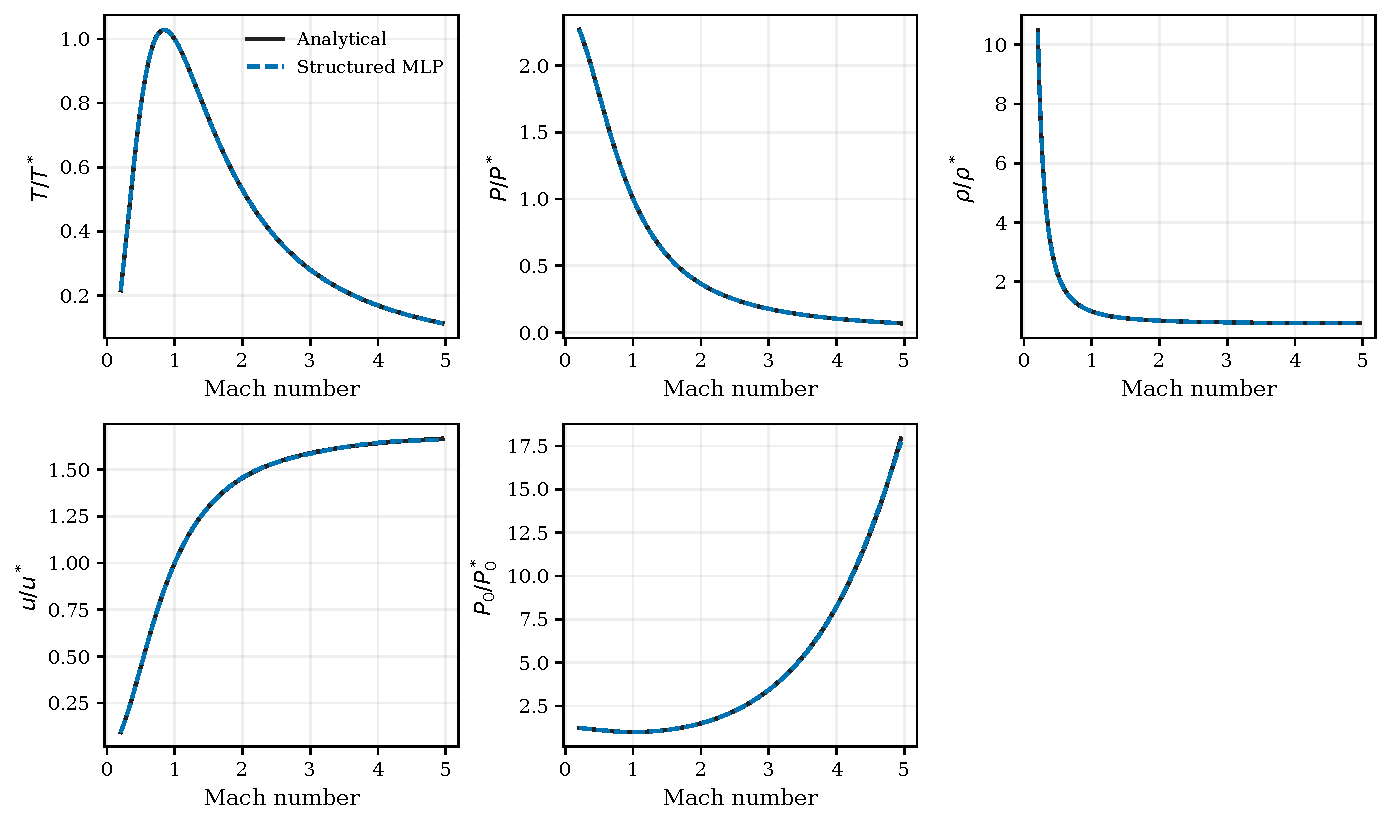
\includegraphics[width=0.9\textwidth]{Rayleigh_Comparison_Revised.pdf}
    \caption{Detailed comparison of Rayleigh flow properties. The neural network captures the specific nonlinear behavior of each property ratio, including the velocity increase and density decrease associated with heat addition in subsonic flow.}
    \label{fig:rayleigh_comparison}
\end{figure}

\begin{revision}
Table~\ref{tab:rayleigh_forward_error} quantifies the forward comparison. For each property vector $\mathbf y$ evaluated at 1,000 independent logarithmically spaced Mach numbers over $0.205\le M\le4.95$, the reported norms are $\|\widehat{\mathbf y}-\mathbf y\|_2/\|\mathbf y\|_2$ and $\|\widehat{\mathbf y}-\mathbf y\|_\infty/\|\mathbf y\|_\infty$. The separate inverse blind-grid norms are reported later in Table~\ref{tab:primary_metrics}.

\begin{table}[H]
\centering
\caption{Rayleigh forward-model error on the independent 1,000-state evaluation grid.}
\label{tab:rayleigh_forward_error}
\small
\begin{tabular}{lrr}
\toprule
Predicted ratio & Relative $L_2$ error (\%) & Relative $L_\infty$ error (\%) \\
\midrule
$T/T^*$       & 0.1022 & 0.1292 \\
$P/P^*$       & 0.0521 & 0.1065 \\
$\rho/\rho^*$ & 0.3004 & 0.7669 \\
$u/u^*$       & 0.1294 & 0.4357 \\
$P_0/P_0^*$   & 0.4769 & 1.1408 \\
\bottomrule
\end{tabular}
\end{table}
\end{revision}

\subsubsection{The Inverse Problem}
The inverse problem—determining the Mach number for a given temperature ratio—is a common task in gas-dynamics analysis. Since analytical inversion of the implicit Rayleigh equations is unavailable in a convenient single-valued form, users typically rely on tables or iterative solvers. Our "Expert Networks" approach provides a direct branch-declared solution. Figure \ref{fig:rayleigh_inverse} visualizes this inverse mapping. The grey line represents the analytical solution, while the red and blue dashed lines show the predictions of the subsonic and supersonic networks, respectively. \rev{The inverse uses the stagnation-temperature relation:}

\begin{equation}
    \frac{T_0}{T_0^*} = \frac{2(\gamma+1)M^2\left(1+\frac{\gamma-1}{2}M^2\right)}{(1+\gamma M^2)^2}.
\end{equation}

This clearly demonstrates how the branch splitting strategy successfully resolves the non-uniqueness issue.

\begin{figure}[H]
    \centering
    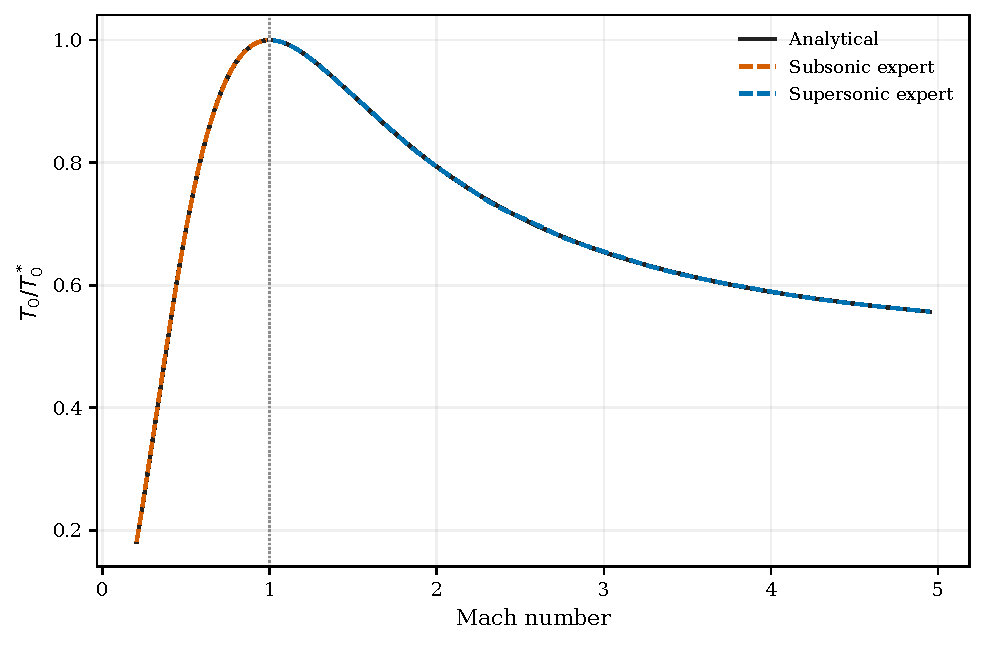
\includegraphics[width=0.8\textwidth]{Rayleigh_Inverse_Revised.pdf}
    \caption{Corrected inverse Rayleigh problem based on $T_0/T_0^*$. The grey curves are analytical; the red and blue dashed curves are the bounded subsonic and supersonic expert predictions.}
    \label{fig:rayleigh_inverse}
\end{figure}

\subsubsection{Thermodynamic Consistency}
The ultimate verification of any gas dynamics model is its adherence to the Second Law of Thermodynamics. We reconstructed the Rayleigh line on a Temperature-Entropy ($T-s$) diagram using the AI-predicted values (Figure \ref{fig:rayleigh_ts}). The entropy change is computed from the predicted pressure and temperature ratios:
\begin{equation}
    \frac{s-s^*}{c_p} = \ln(T/T^*) - \frac{\gamma-1}{\gamma} \ln(P/P^*)
\end{equation}
\rev{The predicted entropy curve reaches its maximum at the same sampled sonic state as the analytical curve; the maximum entropy-value discrepancy is 0.0205 in the reported nondimensional measure. This is a consistency diagnostic, not proof that every conservation identity is enforced exactly.}

\begin{figure}[H]
    \centering
    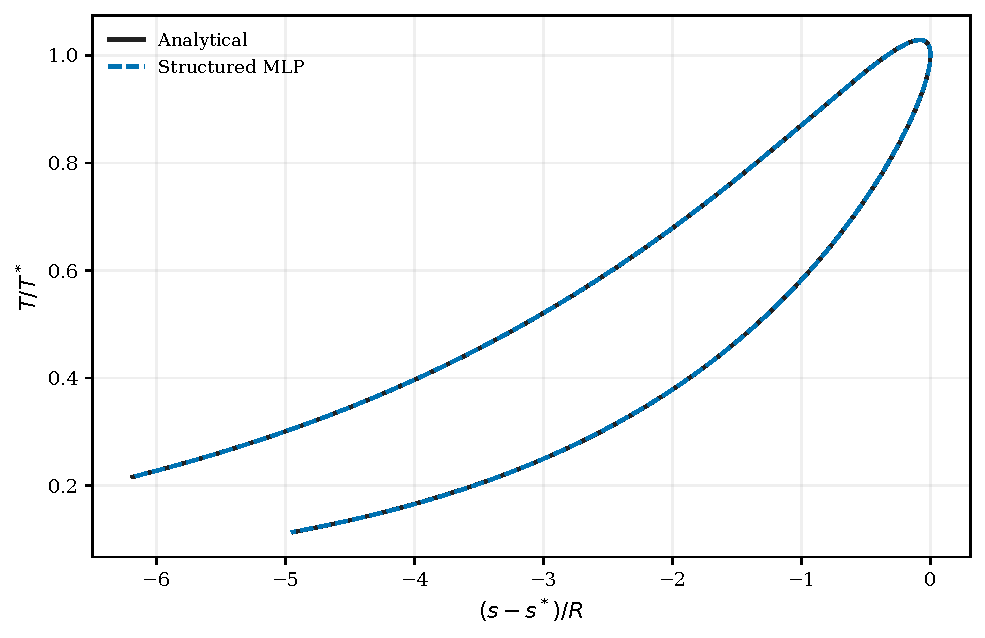
\includegraphics[width=0.8\textwidth]{Rayleigh_Ts_Revised.pdf}
    \caption{The Rayleigh line on a T-s diagram generated by the neural network. The model correctly identifies the point of maximum entropy ($M=1$), consistent with the Second Law of Thermodynamics. The arrow indicates the direction of heat addition driving the flow towards the sonic state.}
    \label{fig:rayleigh_ts}
\end{figure}


\subsection{Fanno Flow: Adiabatic Flow with Friction}
Fanno flow describes the adiabatic flow of a compressible fluid through a constant-area duct with friction. It is governed by the conservation of mass, momentum, and energy, combined with the equation of state. The key challenge in Fanno flow is the implicit relationship between the Mach number ($M$) and the friction parameter ($4fL^*/D$), as well as the asymptotic behavior of properties as the flow approaches the sonic state ($M=1$).

\subsubsection{Governing Equations and Data Generation}
The analytical relations for property ratios with respect to the sonic reference state (denoted by $*$) are given by:
\begin{align}
    \frac{T}{T^*} &= \frac{\gamma+1}{2+(\gamma-1)M^2} \\
    \frac{P}{P^*} &= \frac{1}{M} \sqrt{\frac{\gamma+1}{2+(\gamma-1)M^2}} \\
    \frac{\rho}{\rho^*} &= \frac{1}{M} \sqrt{\frac{2+(\gamma-1)M^2}{\gamma+1}} \\
    \frac{P_0}{P_0^*} &= \frac{1}{M} \left( \frac{2+(\gamma-1)M^2}{\gamma+1} \right)^{\frac{\gamma+1}{2(\gamma-1)}} \\
    \frac{4fL^*}{D} &= \frac{1-M^2}{\gamma M^2} + \frac{\gamma+1}{2\gamma} \ln\left( \frac{(\gamma+1)M^2}{2+(\gamma-1)M^2} \right)
\end{align}
\rev{The experiment uses 900 analytical training states over $0.2\le M\le5.0$, combining logarithmic Mach sampling with additional points near $M=1$. The inverse test grid contains 1,040 independent states and is logarithmically refined near the sonic limit.}

\subsubsection{Machine Learning Architecture}
Within the general MLP framework introduced earlier, the Fanno problem requires additional target and feature transformations because the friction parameter spans several orders of magnitude and approaches zero quadratically at $M=1$. As in the Rayleigh case, the Fanno problem is decomposed into distinct forward and inverse learning tasks rather than being handled through a single universal network.

\begin{revision}
The forward formulation imposes the known sonic structure explicitly,
\begin{equation}
\widehat{\frac{4fL^*}{D}}=(M-1)^2\exp[g_\theta(M)],
\label{eq:fanno_positive_transform}
\end{equation}
where $g_\theta$ is learned from the features $(M,\log M,M^2)$. Equation~\ref{eq:fanno_positive_transform} makes the prediction non-negative and exactly zero at $M=1$. The four positive thermodynamic ratios are learned in logarithmic coordinates. For inversion, two $32\times32$ Tanh experts receive $\sqrt{4fL^*/D}$ and return bounded Mach coordinates on the subsonic and supersonic intervals. The same optimizer and stopping criteria as Table~\ref{tab:training_contract} are used. This representation, rather than a claim of universal superiority for a particular activation function, is the principal source of near-sonic stability.
\end{revision}



\subsubsection{Results: Property Ratios}

Figure \ref{fig:fanno_ratios} compares the direct neural-network predictions with the analytical Fanno ratios over $0.2\le M\le5.0$. Quantitative blind inverse errors and physical diagnostics are reported in Tables~\ref{tab:primary_metrics} and~\ref{tab:ablation_physics} rather than inferred from visual overlap alone.

The physical interpretation of the plots indicates that the temperature ratio for an ideal gas with $\gamma = 1.4$ starts from about 1.2 at the stagnant state and decreases monotonically as Mach number increases. This is expected because, in Fanno flow with constant total enthalpy, friction accelerates the flow and increases the kinetic energy; consequently, the static temperature must decrease to satisfy energy conservation.

The static-pressure plot also reveals that, in low subsonic speeds, pressure tends to infinity, reflecting the singularity of the sonic reference state relative to the stagnation condition. The model successfully captures this steep gradient in the subsonic region and the more gradual pressure decrease in the supersonic regime. The density behavior follows a similar trend, decreasing monotonically since, in a constant-area duct, density is inversely related to velocity; the model accurately reproduces this hyperbolic relationship.

In the velocity plot, the curve begins at zero and crosses the value of one at Mach 1, demonstrating the non-intuitive nature of Fanno flow, where friction accelerates subsonic flow but decelerates supersonic flow. 

Finally, the most important thermodynamic confirmation appears in the stagnation-pressure ratio plot, which exhibits a global minimum equal to one at Mach 1. The convex shape shows that any deviation from the sonic condition leads to a higher stagnation pressure relative to the critical state. The neural network successfully models this curvature and its minimum with high precision, demonstrating that the model implicitly respects the second law of thermodynamics and correctly captures entropy production.


\begin{figure}[H]
    \centering
    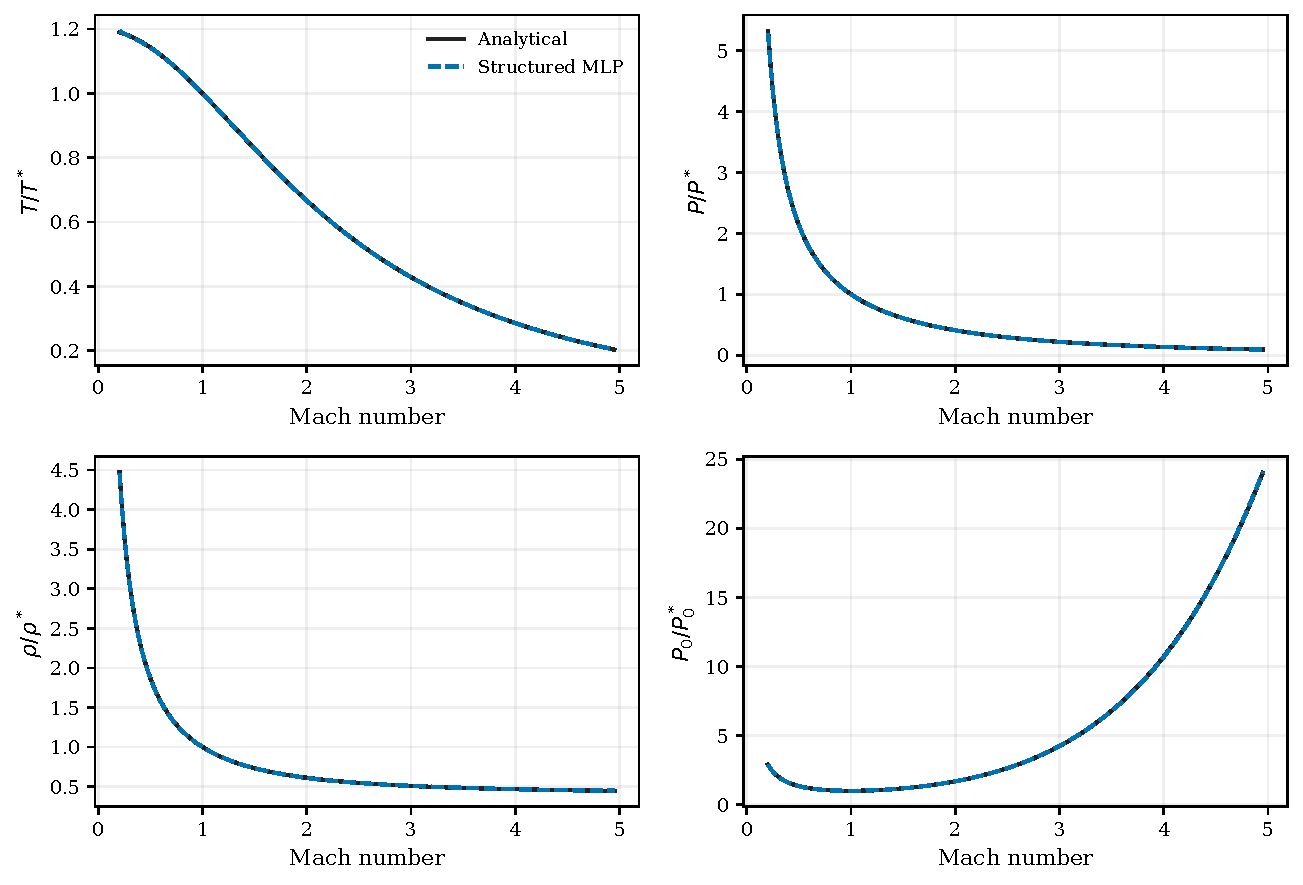
\includegraphics[width=0.95\textwidth]{Fanno_Ratios_Revised.pdf}
    \caption{Comparison of analytical vs. neural network predictions for Fanno flow property ratios. The model accurately captures the divergent behavior of pressure and density at low Mach numbers and the extremum at M=1.}
    \label{fig:fanno_ratios}
\end{figure}

\subsubsection{Handling the Fanno Friction Singularity}
The prediction of the Fanno friction parameter, $4fL^*/D$, given by eq. (13), presents a unique computational challenge due to its mathematical structure:
As the Mach number approaches zero ($M \to 0$), the first term dominates, causing the parameter to approach infinity asymptotically ($\propto M^{-2}$). Conversely, at the sonic state ($M=1$), the value drops to zero. This creates a target variable that spans several orders of magnitude (from $10^5$ to $10^{-5}$), causing standard regression models to fail. A neural network trained on the raw values would suffer from exploding gradients in the subsonic regime and vanishing sensitivity in the supersonic regime.

\rev{A raw-output MLP is not reliable in this limit: in the controlled audit over $|M-1|<0.05$, it predicts a negative friction-length value for 96.9\% of the sampled states. The structured model in Equation~\ref{eq:fanno_positive_transform} has zero invalid outputs by construction and a local MAE of $1.23\times10^{-8}$. Figure~\ref{fig:fanno_friction} retains the original friction-curve presentation, while the numerical ablation is reported in Table~\ref{tab:ablation_physics}.}

\begin{figure}[H]
    \centering
    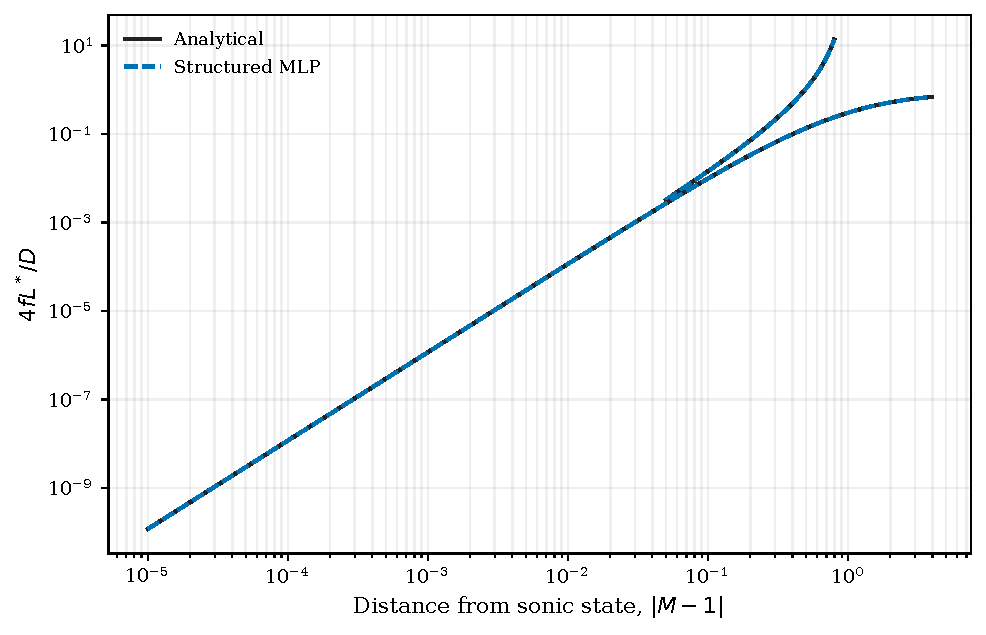
\includegraphics[width=0.8\textwidth]{Fanno_Friction_Revised.pdf}
    \caption{Prediction of the Fanno friction parameter. The distance-to-sonic logarithmic axes expose the exact quadratic decay, which is built into the structured output.}
    \label{fig:fanno_friction}
\end{figure}



\subsubsection{The Inverse Problem: Direct Mach Prediction}

In practical engineering design, the duct geometry (length $L$ and diameter $D$) and friction factor ($f$) are often fixed constraints, requiring the determination of the flow Mach number ($M$). The governing Fanno flow equation relates the friction parameter $\frac{4fL^*}{D}$ to the Mach number as follows:

\begin{equation}
    \frac{4fL^*}{D} = \frac{1-M^2}{\gamma M^2} + \frac{\gamma+1}{2\gamma}\ln\left(\frac{(\gamma+1)M^2}{2+(\gamma-1)M^2}\right)
    \label{eq:fanno_friction}
\end{equation}

Equation \ref{eq:fanno_friction} is highly non-linear and implicit with respect to $M$. Conventional methods rely on iterative numerical solvers (e.g., Newton-Raphson) or look-up tables to solve for $M$, which can be computationally expensive in large-scale simulations. Furthermore, the function is non-bijective; for a given value of the friction parameter (limit $\frac{4fL^*}{D} < \frac{4fL^*_{max}}{D}$), there exist two distinct mathematical solutions for $M$: one in the subsonic regime ($M < 1$) and one in the supersonic regime ($M > 1$).

To address this ill-posedness and eliminate iterative costs, we propose a domain-decomposed neural approach. The solution space is split into subsonic and supersonic regimes. \rev{Two specialized experts learn an inverse relation whose input is $\sqrt{4fL^*/D}$ and whose output is $M$. Their latent outputs are mapped into the respective admissible Mach intervals. The square-root input follows the local quadratic sonic behavior and remains finite at choking.}

For quantitative validation of the inverse surrogate, Figure~\ref{fig:inverse_fanno} compares the branch-wise neural-network predictions against the analytical Fanno relation over both the subsonic and supersonic regimes. The logarithmic horizontal axis highlights the wide dynamic range of the friction parameter and demonstrates that the learned inverse mappings remain accurate both near the choking point and in the asymptotic low-Mach region.

\begin{figure}[htbp]
    \centering
    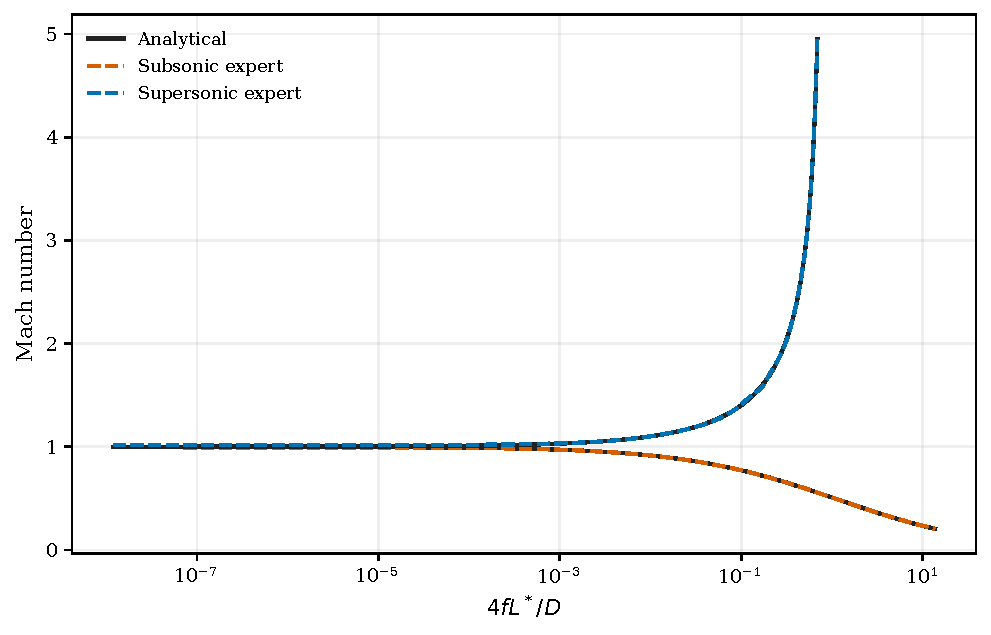
\includegraphics[width=0.8\linewidth]{Fanno_Inverse_Revised.pdf}
    \caption{Analytical and bounded expert solutions of the inverse Fanno relation on the subsonic and supersonic branches. The logarithmic abscissa resolves the approach to the sonic state.}
    \label{fig:inverse_fanno}
\end{figure}

\subsubsection{Thermodynamic Consistency and Case Study}
Finally, we verify the thermodynamic consistency of the model by plotting the Fanno line on a Temperature-Entropy ($T-s$) diagram (Figure \ref{fig:fanno_ts}). The entropy change is calculated using the AI-predicted $P$ and $T$:
\begin{equation}
    \frac{s-s^*}{c_p} = \ln(T/T^*) - \frac{\gamma-1}{\gamma} \ln(P/P^*)
\end{equation}
\rev{The sampled maximum-entropy location agrees with the analytical sonic state, while the maximum entropy-value discrepancy is 0.0175. This supports thermodynamic consistency but does not imply exact enforcement of every governing identity.} Furthermore, Figure \ref{fig:fanno_solution} visualizes a specific case study: a supersonic flow at $M=2.5$ entering a duct. The AI solver computes the path along the Fanno line towards the sonic state, providing a clear visual aid for users.

\begin{figure}[H]
    \centering
    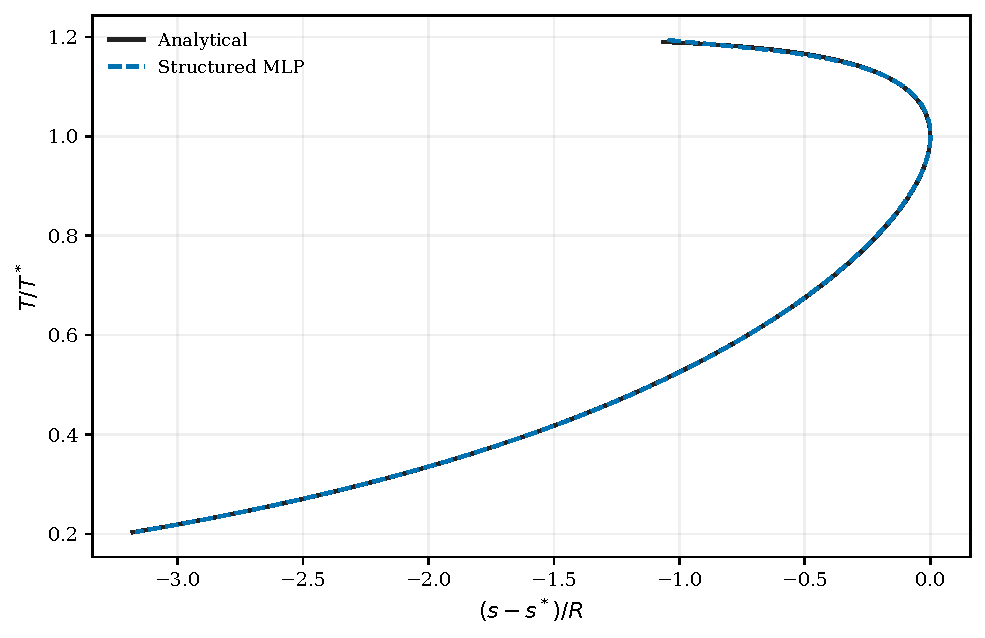
\includegraphics[width=0.8\textwidth]{Fanno_Ts_Revised.pdf}
    \caption{The Fanno line on a T-s diagram generated by the neural network. The curve correctly shows the entropy maximization point at the sonic state.}
    \label{fig:fanno_ts}
\end{figure}

\begin{figure}[H]
    \centering
    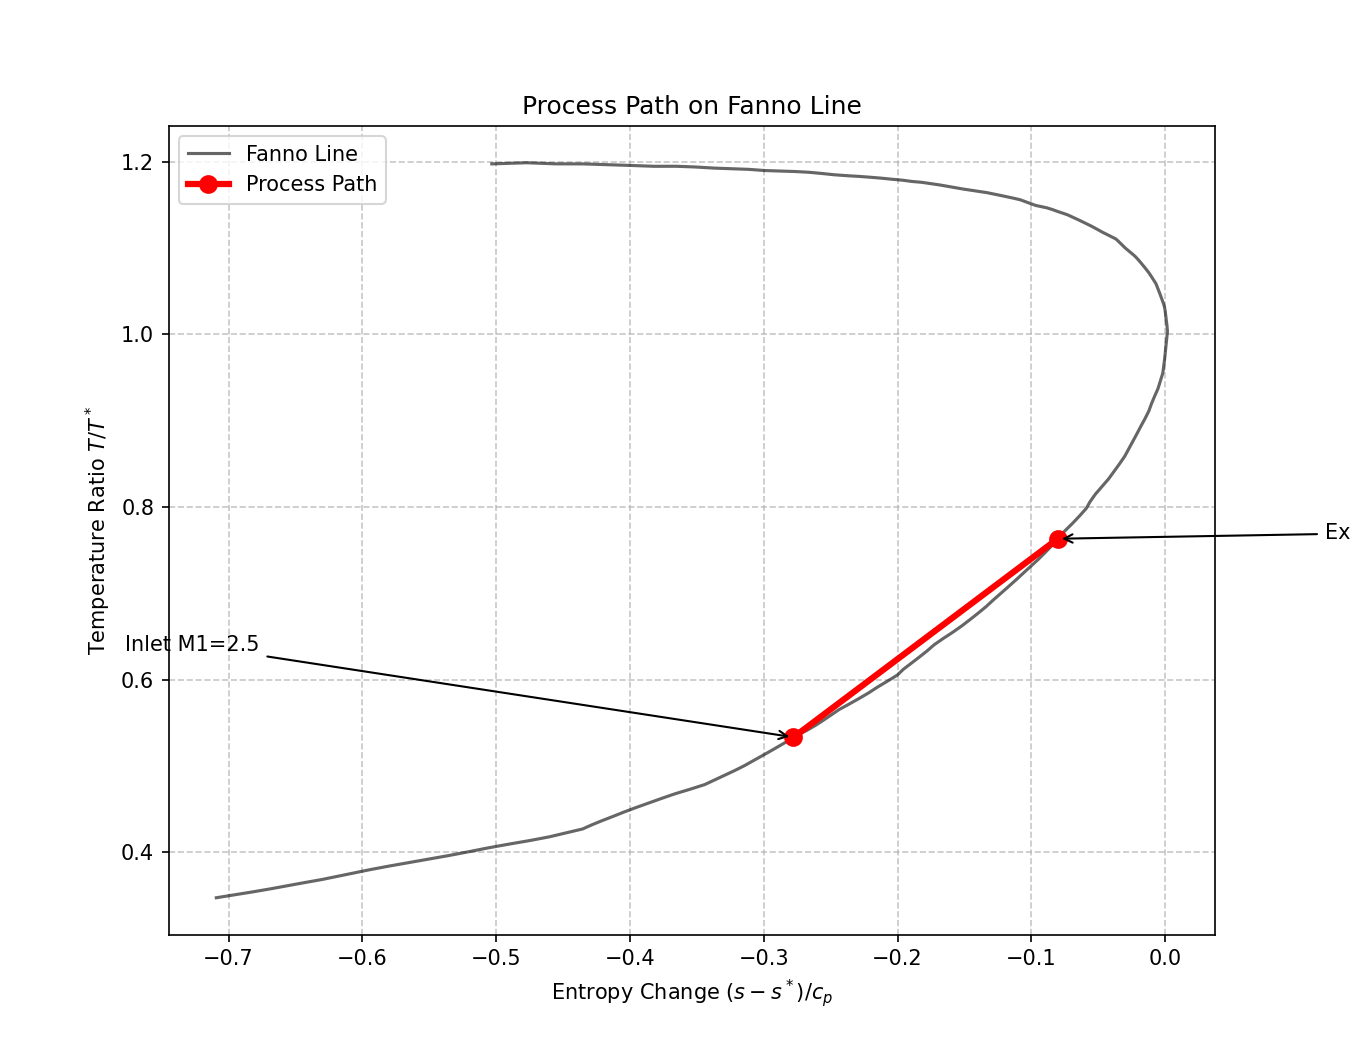
\includegraphics[width=0.82\textwidth]{Fanno_Process_Path.png}
    \caption{Case-study visualization of the process path on the Fanno line for a supersonic inlet condition. The AI surrogate predicts the exit state and reconstructs the thermodynamic path on the $T$--$s$ plane, illustrating the progression of the flow toward the sonic condition under friction.}
    \label{fig:fanno_solution}
\end{figure}

\subsection{Oblique Shocks: The \texorpdfstring{$\beta-\theta-M$}{beta-theta-M} Manifold}

The interaction of a supersonic flow with a concave corner generates an oblique shock wave, a fundamental phenomenon in compressible aerodynamics. This interaction is governed by the strictly non-linear $\beta-\theta-M$ relation, which couples the upstream Mach number ($M_1$), the shock wave angle ($\beta$), and the flow deflection angle ($\theta$).

For a calorically perfect gas with a specific heat ratio $\gamma$, the governing equation is given by:

\begin{equation}
    \tan \theta = 2 \cot \beta \left[ \frac{M_1^2 \sin^2 \beta - 1}{M_1^2 (\gamma + \cos 2\beta) + 2} \right]
    \label{eq:beta_theta_m}
\end{equation}

Equation \ref{eq:beta_theta_m} defines a complex, non-bijective surface (manifold) in 3D space. While solving for the deflection angle $\theta$ given $M_1$ and $\beta$ is a direct algebraic calculation, the inverse problem—finding the shock angle $\beta$ for a specific geometry ($\theta$) and flight condition ($M_1$)—is implicit and requires iterative numerical methods.

The solution space is constrained by critical physical boundaries that standard regression models frequently fail to capture without physics-informed constraints:

\begin{itemize}
    \item The Mach Wave Limit ($\beta \to \mu$): As the deflection angle approaches zero ($\theta \to 0$), the shock wave weakens to an isentropic Mach wave. The shock angle converges to the Mach angle $\mu = \arcsin(1/M_1)$. Pure data-driven models often struggle here, predicting non-zero shock strengths where no discontinuity should exist.
    
    \item The Detachment Limit ($\theta_{max}$): For any given Mach number, there exists a maximum deflection angle $\theta_{max}$ beyond which Equation \ref{eq:beta_theta_m} yields no real roots. Physically, this corresponds to shock detachment, where the oblique shock transforms into a curved bow shock. 
    
    \item Solution Duality (Strong vs. Weak): For any valid pair of $M_1$ and $\theta < \theta_{max}$, there are two mathematical solutions for $\beta$: the \textit{weak solution} (prevalent in external aerodynamics) and the \textit{strong solution} (typically found in internal flows or high-backpressure scenarios).
\end{itemize}

Modeling this manifold presents a unique challenge for neural networks. A standard Mean Squared Error (MSE) loss function tends to average the weak and strong solutions near the $\theta_{max}$ turning point, resulting in physically invalid predictions that lie off the manifold. Furthermore, the steep gradients near the detachment point require high sampling density to prevent "corner-cutting" by the regression surface. 


\subsubsection{ML Strategy: Boundary Envelope and Branch Experts}

Standard data-driven regression models often struggle to enforce exact boundary conditions, leading to non-zero residuals at theoretical limits. The Mach-wave limit is defined by

\begin{equation}
    \beta_{min} = \mu = \arcsin\left(\frac{1}{M}\right)
\end{equation}

\begin{revision}
Endpoint samples alone act as \emph{soft} data anchors rather than hard constraints. The direct model therefore defines $q=(\beta-\mu)/(\pi/2-\mu)$ and
\begin{equation}
\widehat{\theta}=q(1-q)\exp[h_\theta(M,q)],
\label{eq:oblique_envelope}
\end{equation}
which enforces $\widehat{\theta}=0$ at both the Mach-wave and normal-shock endpoints. The inverse task is learned separately: a $64\times64$ Tanh MLP returns weak and strong latent coordinates that are mapped into $(\mu,\pi/2)$ and checked for the ordering $\beta_{\rm weak}<\beta_{\rm strong}$. A naive single-output inverse receives duplicate $(M,\theta)$ inputs paired with incompatible labels and therefore averages between branches; the quantitative ablation is given in Table~\ref{tab:ablation_physics}.
\end{revision}



The network architecture for the oblique-shock surrogate was selected to provide sufficient expressive capacity for the strongly curved $\beta$--$\theta$--$M$ manifold while maintaining training stability. \rev{The direct and inverse models use 900 analytical training states and the common protocol in Table~\ref{tab:training_contract}.}

\subsubsection{Results: Reconstruction of the Shock Manifold}

Figure \ref{fig:beta_theta} presents the superposition of the AI-predicted shock polars against the analytical exact solution. The neural network demonstrates high-fidelity agreement across the entire supersonic regime, effectively reconstructing the complex topology of the $\beta-\theta-M$ manifold.

Three key performance indicators are evident in these results:

\begin{enumerate}
    \item Resolution of Solution Duality: \rev{The dedicated inverse outputs distinguish the weak and strong solutions. On the blind grid, their combined MAE is $5.08\times10^{-4}$ rad with 100\% correct branch ordering; a naive single-output inverse has a branch-distance MAE of 0.4246 rad.}
    
    \item Locus of Maximum Deflection ($\theta_{max}$): The peaks of the curves, representing the critical detachment angle $\theta_{max}$ for each Mach number, are identified with high precision. This is computationally significant, as the gradient of the function $\partial \theta / \partial \beta$ becomes zero at these points, historically causing instability in standard regression techniques. The AI model accurately delimits the boundary between attached oblique shocks and detached bow shocks.
    
    \item Boundary Consistency: Equation~\ref{eq:oblique_envelope} makes the predicted curves exactly zero at the Mach-wave and normal-shock endpoints; the measured endpoint residual is zero to machine precision.
\end{enumerate}

\rev{The inverse blind-grid relative $L_2$ error is $7.99\times10^{-4}$; local errors increase toward detachment and are reported separately in the repository.}

\begin{figure}[H]
    \centering
    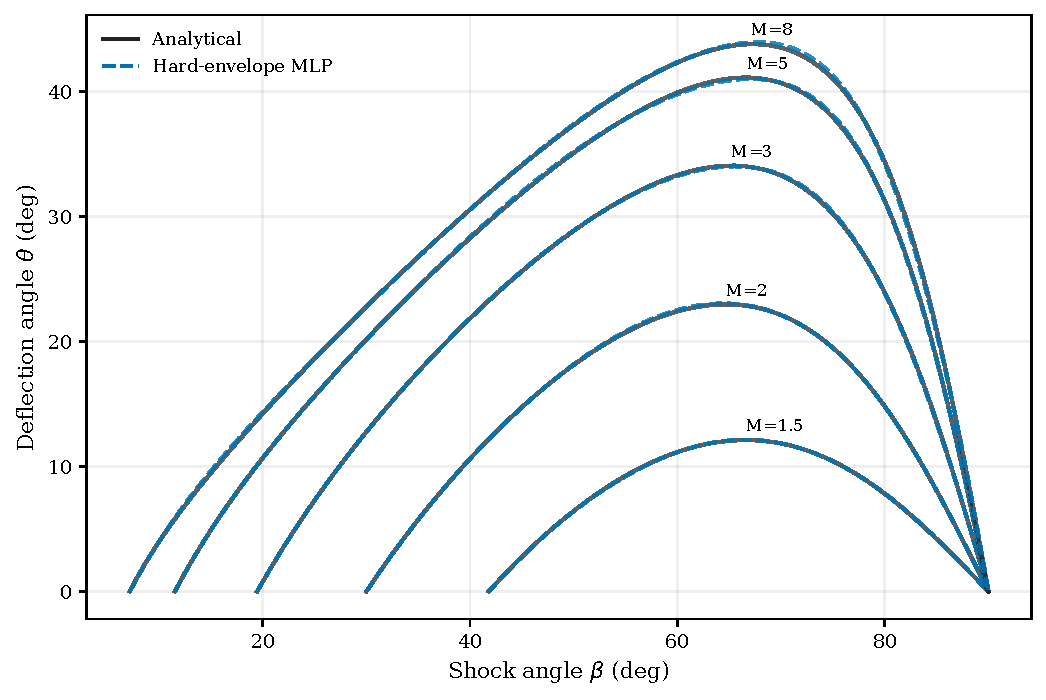
\includegraphics[width=1.0\textwidth]{Oblique_Manifold_Revised.pdf}
    \caption{Constrained $\beta$--$\theta$--$M$ diagram. Dashed curves are the hard-envelope surrogate and solid curves are the analytical relation; both physical endpoints are imposed exactly.}
    \label{fig:beta_theta}
\end{figure}

\subsection{Normal Shocks in Convergent-Divergent Nozzles}



The operation of a Convergent-Divergent (C-D) nozzle is governed by the pressure ratio across it. When the back pressure ($P_b$) is low enough to choke the throat ($M_t=1$) but high enough to prevent fully supersonic flow at the exit, a normal shock wave forms inside the divergent section. Locating this shock is a classic and computationally demanding inverse problem in compressible-flow analysis.

The flow physics involves a sequential chain of isentropic expansion, non-isentropic shock compression, and isentropic subsonic diffusion. The fundamental difficulty lies in relating the known boundary conditions (Area Ratio $A_e/A_t$ and Pressure Ratio $P_b/P_{01}$) to the unknown shock location ($A_s/A_t$).

The governing relationship links the total pressure loss across the shock to the geometric area constraints. For a perfect gas, the ratio of stagnation pressures across a normal shock is inversely proportional to the ratio of critical throat areas:

\begin{equation}
    \frac{P_{02}}{P_{01}} = \frac{A_t}{A^*_{2}}
    \label{eq:total_pressure_loss}
\end{equation}

Where $P_{01}$ is the inlet total pressure, $P_{02}$ is the exit total pressure (post-shock), $A_t$ is the physical throat area, and $A^*_{2}$ is the virtual throat area required for the flow to re-choke after the shock.

The exit static pressure $P_e$ (which equals $P_b$ for subsonic exit flow) is related to the shock location via the exit Mach number $M_e$:

\begin{equation}
    \frac{P_b}{P_{01}} = \underbrace{\left( \frac{P_e}{P_{02}} \right)}_{\text{Isentropic Subsonic Exit}} \times \underbrace{\left( \frac{P_{02}}{P_{01}} \right)}_{\text{Shock Strength}}
    \label{eq:chain_rule}
\end{equation}

Since the shock strength depends entirely on the Mach number immediately upstream of the shock ($M_{s1}$), and $M_{s1}$ is determined by the area ratio $A_s/A_t$, Equation \ref{eq:chain_rule} becomes a transcendental function of the shock area $A_s$. Solving for $A_s$ typically requires an iterative "shooting method": guessing a shock location, calculating the resulting pressure loss, and refining the guess until the calculated exit pressure matches the given back pressure.

\subsubsection{ML Strategy: Design Space Mapping}

To bypass the iterative computational cost and provide immediate design feedback, we formulated the shock location problem as a direct regression task. We trained an MLP to approximate the inverse function $\mathcal{F}^{-1}$:

\begin{equation}
    \frac{A_s}{A_t} \approx \text{MLP}\left( \frac{A_e}{A_t}, \frac{P_b}{P_{01}} \right)
\end{equation}

The network maps the design constraints (geometry and back pressure) directly to the physical response (shock area).
\begin{revision}
To prevent a shock prediction outside the divergent section, the raw network coordinate $z$ is transformed as
\begin{equation}
\frac{A_s}{A_t}=1+\sigma(z)\left(\frac{A_e}{A_t}-1\right).
\label{eq:nozzle_bound}
\end{equation}
The $64\times64$ Tanh model is trained on 900 analytical states and tested on 896 independent states.
\end{revision}
This approach "flattens" the iterative physics solver into a single forward-pass operation. \rev{Measured batch timing, rather than an assumed microsecond claim, is reported in Table~\ref{tab:baseline_timing}.}




\subsubsection{Visualization: The Shock Location Heatmap}



The speed of the AI solver enables the real-time generation of a "Design Heatmap" (Figure \ref{fig:nozzle_heatmap}), which visualizes the entire solution space of the nozzle. This diagram plots the Nozzle Area Ratio ($A_e/A_t$) on the x-axis and the Back Pressure Ratio ($P_b/P_{01}$) on the y-axis, with the color contour representing the shock location ($A_s/A_t$).

This visualization highlights several critical flow regimes:
\begin{itemize}
    \item The Valid Shock Domain: The colored region represents the specific combinations of geometry and pressure where a normal shock can physically exist inside the nozzle.
    \item The Throat Limit ($A_s \to A_t$): As back pressure increases (moving up the y-axis), the shock is pushed upstream towards the throat. The heatmap clearly shows the boundary where the shock vanishes and the nozzle unchokes (First Critical Point).
    \item The Exit Limit ($A_s \to A_e$): As back pressure decreases, the shock moves downstream. The lower boundary of the heatmap corresponds to the "Third Critical Point," where the normal shock sits exactly at the exit plane. Below this line, the flow becomes over-expanded with oblique shocks outside the nozzle.
\end{itemize}

By exploring this heatmap, users can intuitively grasp how sensitive the shock position is to small changes in back pressure, a concept that is often obscured by single-point algebraic calculations.

\begin{figure}[H]
    \centering
    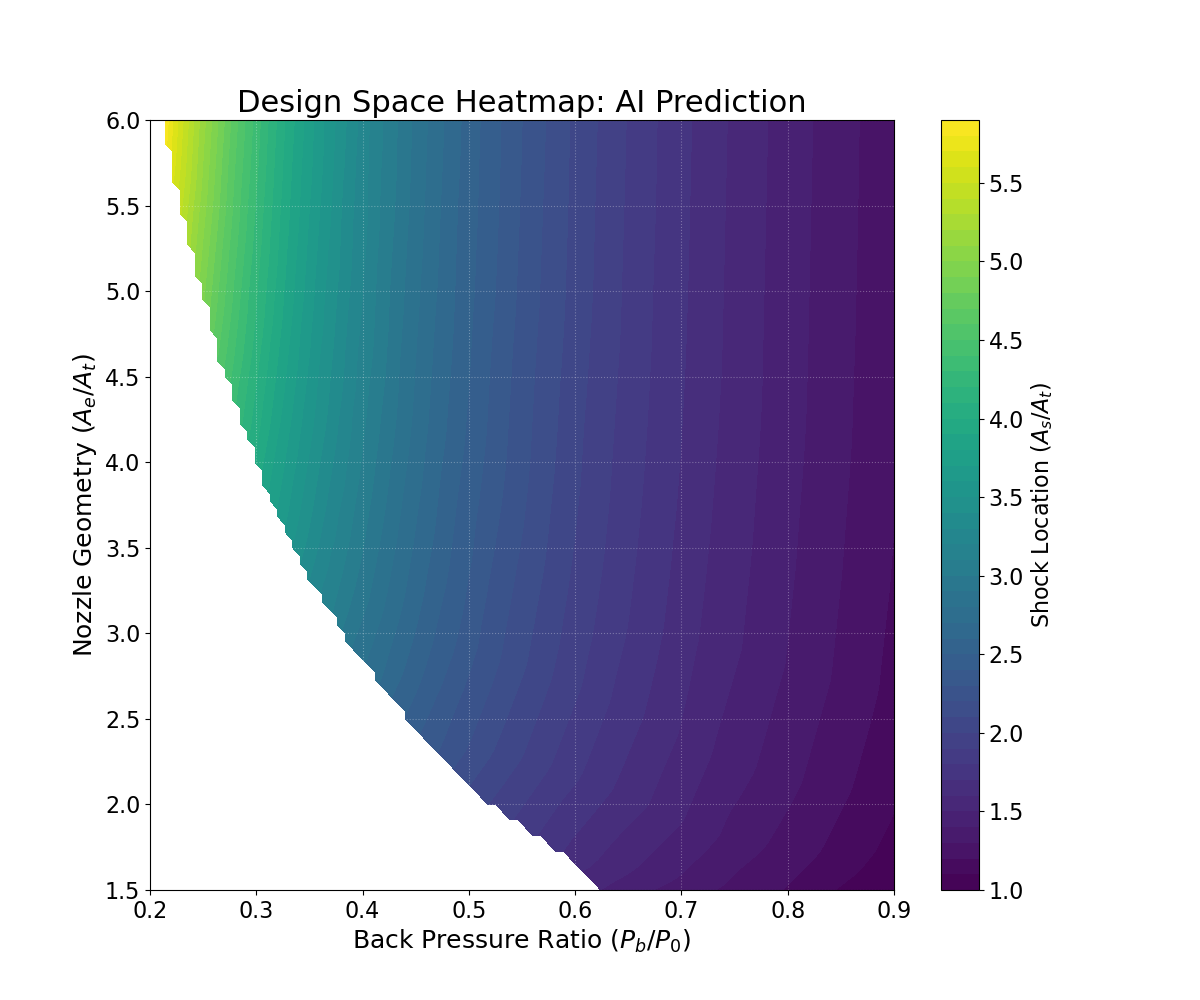
\includegraphics[width=0.9\textwidth]{design_heatmap.png}
    \caption{Design-space map of the internal shock location. Nozzle exit-area ratio is on the horizontal axis, back-pressure ratio on the vertical axis, and color denotes the predicted internal shock location.}
    \label{fig:nozzle_heatmap}
\end{figure}

\subsubsection{Results: Pressure Distribution Reconstruction}

We coupled the AI shock locator with an analytical reconstructor to generate the pressure distribution along the nozzle (Figure~\ref{fig:nozzle_pressure}). This figure compares the exact analytical solution (solid lines) with the AI-based reconstruction (dashed lines) for the static pressure ratio, $P/P_{0}$, along the nozzle axis. The results correspond to a fixed nozzle geometry with an area ratio of $A_{e}/A_{t} = 3.0$, evaluated under various back-pressure conditions ranging from $P_{b}/P_{0} = 0.4$ to $0.8$.


The plot clearly illustrates the sequence of flow processes: isentropic expansion in the convergent and initial divergent sections, followed by a sharp, discontinuous pressure rise across a normal shock wave, and finally, isentropic subsonic compression to match the exit boundary condition. As expected physically, increasing the back pressure forces the shock wave to move upstream towards the nozzle throat. \rev{On the independent inverse grid, the shock-location model has relative $L_2$ error $1.94\times10^{-3}$, maximum absolute error 0.0229 in $A_s/A_t$, and 100\% valid internal locations because of Equation~\ref{eq:nozzle_bound}.}

\begin{figure}[H]
    \centering
    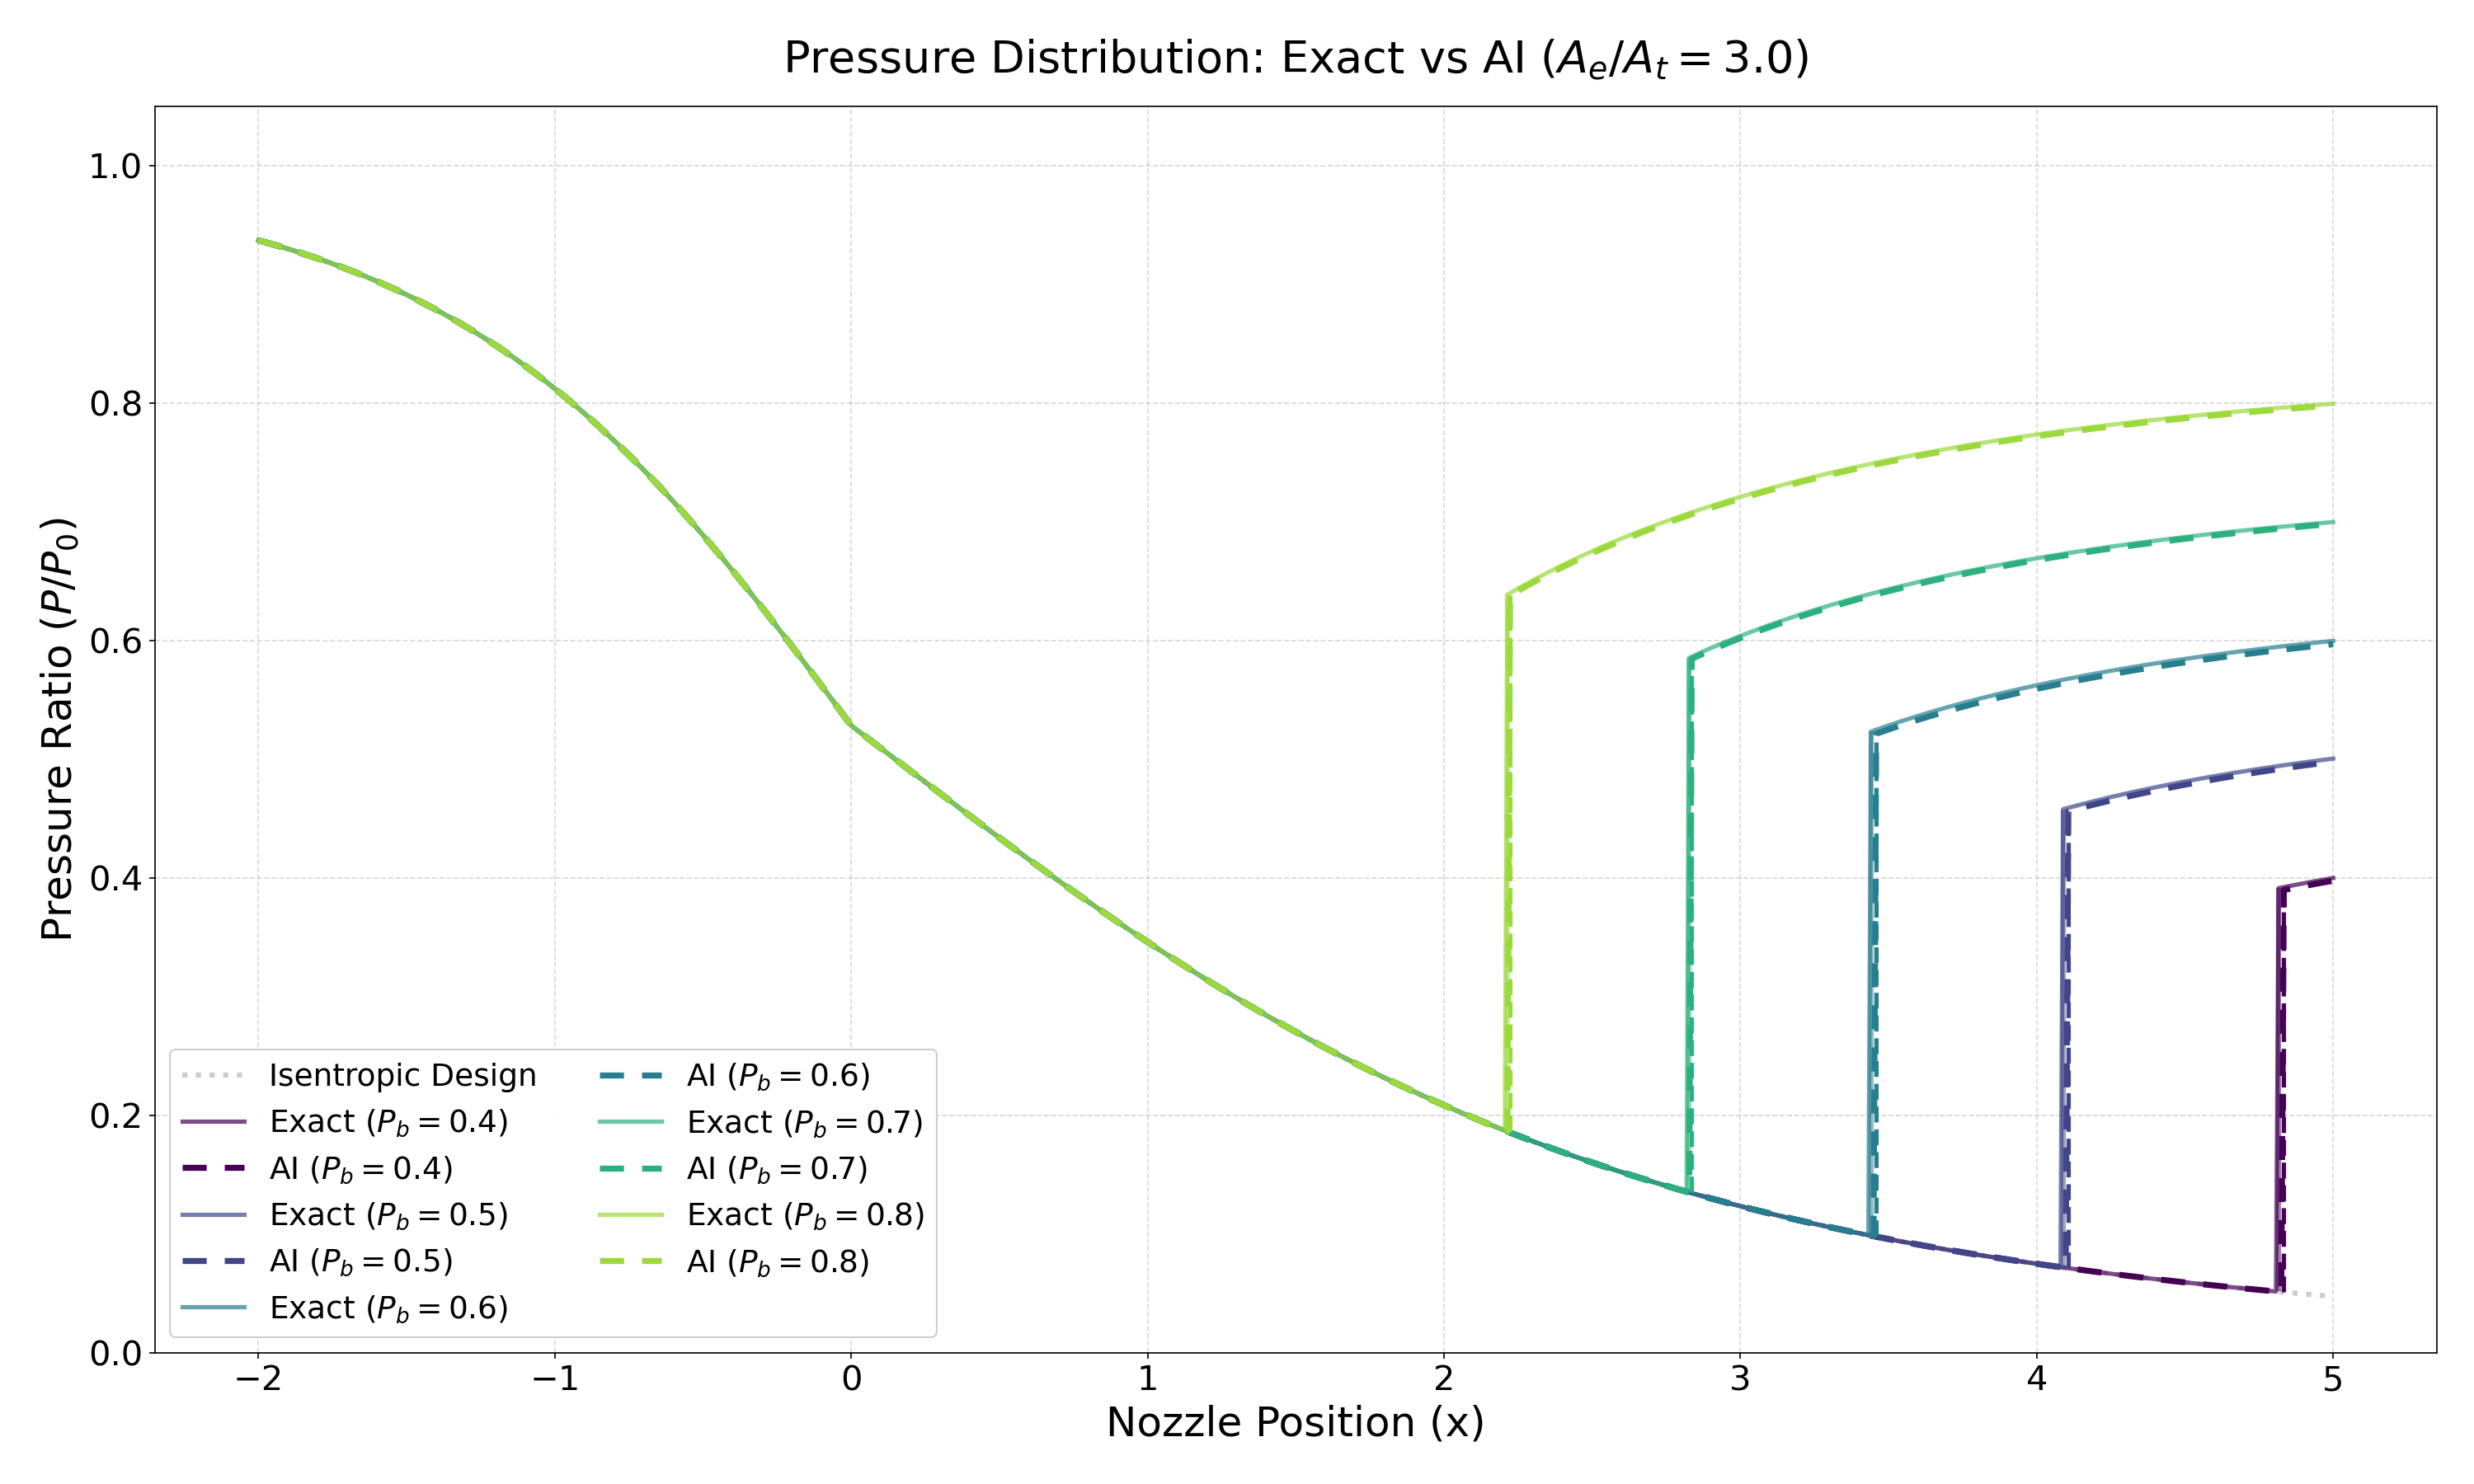
\includegraphics[width=1.0\textwidth]{Nozzle_Pressure_Profiles.png}
    \caption{Pressure distribution along the nozzle axis. The solid lines represent the exact analytical solution, while dashed lines represent the AI reconstruction. The model accurately predicts the shock position for various back-pressures.}
    \label{fig:nozzle_pressure}
\end{figure}

\subsection{Unsteady Shock Tubes: The Riemann Problem}

The shock tube problem constitutes a fundamental benchmark in compressible fluid dynamics, representing the simplest case of unsteady, one-dimensional wave interaction. Physically, it consists of a high-pressure "driver" gas (Region 4) separated from a low-pressure "driven" gas (Region 1) by a diaphragm. Upon the instantaneous rupture of the diaphragm, a shock wave propagates into the low-pressure region, while an expansion fan propagates back into the high-pressure region.

This configuration is mathematically governed by the 1D Euler equations. The central challenge lies in determining the strength of the generated shock wave, defined by the pressure ratio $P_{2}/P_{1}$, given the initial diaphragm pressure ratio $P_{4}/P_{1}$. These two ratios are linked via the fundamental shock tube equation, a highly non-linear implicit function derived by matching pressure and velocity across the contact surface:

\begin{equation}
    \frac{P_4}{P_1} = \frac{P_2}{P_1} \left[ 1 - \frac{(\gamma_4-1)(a_1/a_4)(P_2/P_1 - 1)}{\sqrt{2\gamma_1 \left( 2\gamma_1 + (\gamma_1+1)(P_2/P_1 - 1) \right)}} \right]^{-\frac{2\gamma_4}{\gamma_4-1}}
    \label{eq:shock_tube_implicit}
\end{equation}

Where $a$ denotes the speed of sound and $\gamma$ is the specific heat ratio. Equation \ref{eq:shock_tube_implicit} cannot be solved analytically for $P_2/P_1$. \rev{The reference data are generated with a bracketed Brent solve and an explicit residual check, rather than a fixed initial-guess Newton solve. This scalar compatibility solve is required once per initial state; it should not be confused with a CFD solve at every time step.}

\subsubsection{ML Strategy: The Hybrid Solver}

To address the implicit nature of Equation \ref{eq:shock_tube_implicit} without incurring the computational cost of iterative solvers, we developed a "Hybrid AI-Analytical Solver." 

In this architecture, a lightweight MLP serves as a direct function approximator for the inverse of the shock tube equation. The network takes the initial conditions ($P_4/P_1, T_4/T_1$) as inputs and predicts the shock strength $P_2/P_1$. \rev{Both inputs vary in the dataset: $P_4/P_1\in[1.5,300]$ and $T_4/T_1\in[0.5,2]$.}

Crucially, the AI is not tasked with predicting the entire flow field pixel-by-pixel, which often leads to blurred discontinuities in pure computer vision approaches. Instead, the AI output ($P_2/P_1$) is fed into a deterministic analytical reconstruction module. Once $P_2$ is known, the properties in all other regions (Region 2 behind the shock and Region 3 behind the contact surface) become explicit algebraic calculations:

\begin{equation}
    T_2 = T_1 \left[ \frac{P_2}{P_1} \left( \frac{\frac{\gamma+1}{\gamma-1} + \frac{P_2}{P_1}}{1 + \frac{\gamma+1}{\gamma-1} \frac{P_2}{P_1}} \right) \right]
    \label{eq:temp_ratio}
\end{equation}

\begin{revision}
The learned scalar is bounded as
\begin{equation}
\frac{P_2}{P_1}=1+\sigma(z)\left(\frac{P_4}{P_1}-1\right),
\label{eq:shocktube_bound}
\end{equation}
so the predicted pressure lies strictly between the initial driven and driver pressures. The remaining piecewise states are reconstructed analytically. Their conservation properties are therefore inherited conditional on the finite surrogate error in $P_2/P_1$; no claim of infinite precision is made.
\end{revision}

A lightweight neural architecture was sufficient for the shock-tube surrogate because the network is used only for the implicit shock-strength subproblem, while the remaining thermodynamic states and wave trajectories are reconstructed analytically. \rev{The model has two hidden layers of 64 Tanh units, uses 900 training states, and is tested on a 960-state two-parameter grid.}




\subsubsection{Results: Flow Field and Wave Propagation}

The capabilities of the hybrid solver are demonstrated through the reconstruction of instantaneous property profiles and space-time wave histories.


Figure \ref{fig:shock_tube_profile} compares the instantaneous spatial distribution of pressure, temperature, velocity, and Mach number for three distinct driver pressure ratios at the $T_4/T_1=1$ slice. \rev{Over the full two-input blind grid, the implicit-step relative $L_2$ error is $9.49\times10^{-4}$ and the maximum normalized compatibility residual is 0.0438.}



A critical test of any shock tube solver is the resolution of the \textit{Contact Surface} (the interface between the driver gas and the driven gas). Across this interface:
\begin{itemize}
    \item Pressure and Velocity must be continuous ($P_2 = P_3$, $u_2 = u_3$).
    \item Temperature and Density are discontinuous ($T_2 \neq T_3$, $\rho_2 \neq \rho_3$).
\end{itemize}
As highlighted in the temperature plot of Figure \ref{fig:shock_tube_profile}, the AI-driven model successfully captures this subtle physical phenomenon. While the pressure trace is flat across the middle of the tube, the temperature trace shows a sharp step change, confirming that the model effectively distinguishes between the shock wave (which compresses and heats) and the contact surface (which separates gases of different entropies).


\rev{The analytical reconstruction delineates the three primary wave features:}
\begin{enumerate}
    \item The Shock Wave: Propagating to the right into the quiescent medium (Region 1).
    \item The Contact Surface: Following the shock at a lower velocity, marking the boundary between the hot compressed gas and the cold expanded gas.
    \item The Expansion Fan: Propagating to the left into the high-pressure driver (Region 4), characterized by a smooth, continuous gradient of properties rather than a sharp discontinuity.
\end{enumerate}

The expansion-fan head moves at $-a_4$ and its tail at $u_3-a_3$; these wave locations are reconstructed analytically rather than learned as image pixels.

\begin{figure}[H]
    \centering
    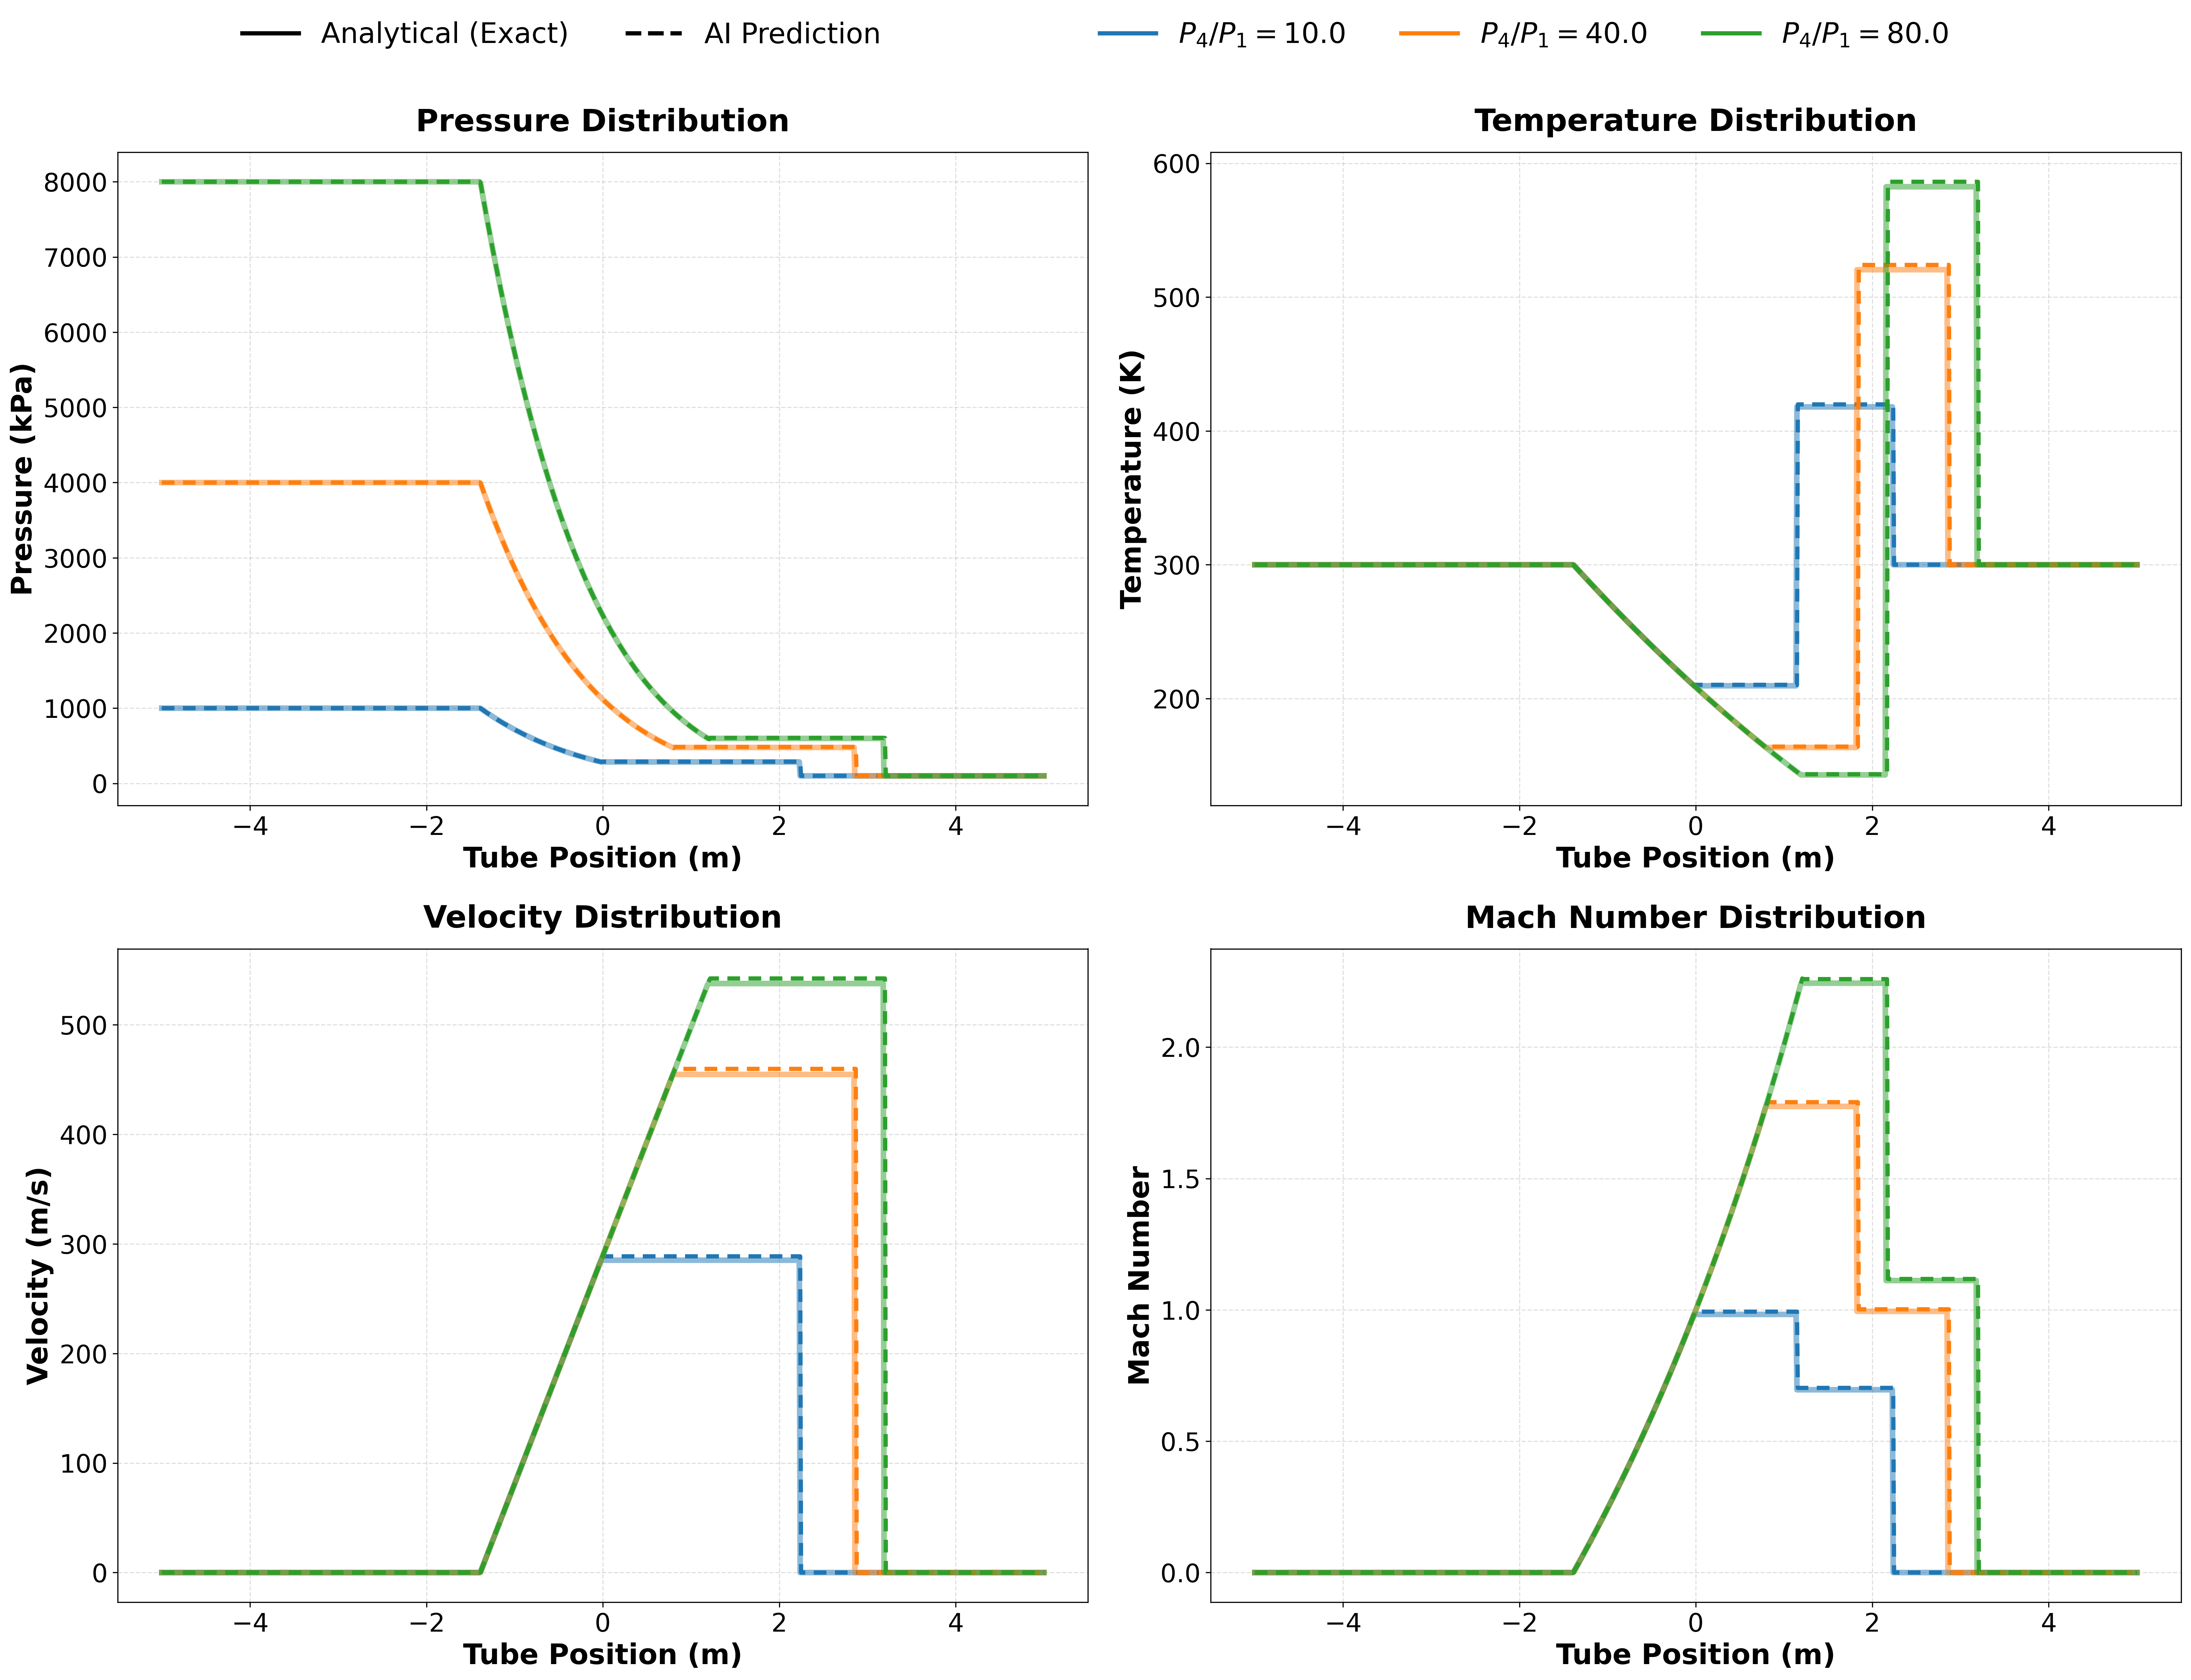
\includegraphics[width=1.0\textwidth]{multi_shock_tube_final.png}
    \caption{Shock tube flow field reconstruction at a specific time step ($t=4ms$). Comparison of AI prediction (dashed) vs. Analytical solution (solid) for pressure ratios of 10, 40, and 80. Note the accurate capture of the contact surface discontinuity in the temperature plot.}
    \label{fig:shock_tube_profile}
\end{figure}




\section{Discussion and Practical Implications}
The examples considered in this work are deliberately canonical, but this choice is central to the purpose of the framework. Canonical gas-dynamics relations provide exact reference solutions, sharply defined physical limits, and well-understood branch structures. They therefore form a reproducible benchmark for the thermal-fluids scientific-machine-learning community, where methods can be tested against nontrivial inverse mappings without ambiguity from numerical discretization, mesh dependence, or solver noise.

The proposed approach should not be interpreted as using neural networks to solve the same physics again in a black-box manner. In each case, the analytical structure is retained and used to define the learning problem. The neural surrogate replaces only the repetitive numerical operation that is inconvenient in practice: inversion of an implicit relation, branch selection, evaluation near a singular limit, or repeated reconstruction over a large parameter sweep. This distinction is important because it separates the present contribution from a simple curve-fitting exercise. The framework is a physics-guided acceleration and packaging strategy for classical relations rather than a substitute for the governing equations.

A purely data-driven or monolithic black-box model would be poorly suited to several of the problems studied here. Rayleigh and Fanno inverse mappings are multi-valued; the Fanno friction parameter spans several orders of magnitude; oblique shocks contain weak and strong branches separated by a detachment limit; and shock-tube solutions require the contact surface, shock, and expansion fan to satisfy different physical constraints. Without branch decomposition, \rev{sonic-coordinate and bounded transformations, exact boundary envelopes}, or hybrid analytical reconstruction, a neural model can average incompatible branches, lose accuracy near sonic or limiting states, or generate physically inconsistent predictions. The success of the present framework therefore comes primarily from physics guidance and problem reformulation, not from increasing network depth or treating the system as an unconstrained regression task.

\begin{revision}
\subsection{Quantitative validation, robustness, and classical baselines}

For $N$ blind targets, the reported relative norms are
\begin{equation}
\relLtwo=\frac{\|\widehat{\mathbf y}-\mathbf y\|_2}{\|\mathbf y\|_2},\qquad
\relLinf=\frac{\|\widehat{\mathbf y}-\mathbf y\|_\infty}{\|\mathbf y\|_\infty}.
\end{equation}
Table~\ref{tab:primary_metrics} quantifies the five principal inverse tasks. These finite errors replace qualitative phrases such as ``near-perfect'' or ``infinite precision.''

\begin{table}[H]
\centering
\caption{Blind inverse-task errors for the physics-guided MLPs.}
\label{tab:primary_metrics}
\small
\begin{tabular}{lrrrr}
\toprule
Problem & $\relLtwo$ & $\relLinf$ & MAE & Maximum absolute error \\
\midrule
Rayleigh inverse & 1.642e-3 & 2.521e-3 & 2.227e-3 & 1.248e-2 \\
Fanno inverse & 3.431e-3 & 3.761e-3 & 4.378e-3 & 1.862e-2 \\
Oblique inverse & 7.990e-4 & 4.543e-3 & 5.076e-4 & 7.116e-3 \\
Nozzle inverse & 1.936e-3 & 4.756e-3 & 3.522e-3 & 2.288e-2 \\
Shock-tube implicit step & 9.490e-4 & 4.209e-3 & 2.388e-3 & 5.373e-2 \\
\bottomrule
\end{tabular}
\end{table}

Table~\ref{tab:ablation_physics} isolates the principal failure modes and the selected physical checks. The hard transforms guarantee only the stated bounds; they do not enforce every conservation identity.

\begin{table}[H]
\centering
\caption{Controlled ablations and physical diagnostics.}
\label{tab:ablation_physics}
\small
\begin{tabular}{p{3.0cm}p{5.3cm}p{3.0cm}}
\toprule
Case & Diagnostic & Result \\
\midrule
Fanno raw output & Negative rate for $|M-1|<0.05$ & 96.9\% \\
Fanno structured output & Negative rate / local MAE & 0\% / $1.23\times10^{-8}$ \\
Oblique naive inverse & Distance to nearest physical branch, MAE & 0.4246 rad \\
Oblique branch experts & MAE / correct ordering & $5.08\times10^{-4}$ rad / 100\% \\
Rayleigh entropy & Maximum value discrepancy / peak-$M$ error & 0.0205 / 0 \\
Fanno entropy & Maximum value discrepancy / peak-$M$ error & 0.0175 / 0 \\
Nozzle & Back-pressure residual / valid location rate & 0.00449 / 100\% \\
Shock tube & Normalized compatibility residual / valid pressure rate & 0.0438 / 100\% \\
\bottomrule
\end{tabular}
\end{table}

Training variability is estimated using seeds 11, 29, and 47. The mean$\pm$standard-deviation $\relLtwo$ values are $(1.49\pm0.65)\times10^{-3}$ for Rayleigh, $(2.36\pm0.33)\times10^{-3}$ for Fanno, $(0.941\pm0.093)\times10^{-3}$ for oblique shocks, $(1.68\pm0.55)\times10^{-3}$ for the nozzle, and $(1.42\pm0.37)\times10^{-3}$ for the shock tube. These values describe ensemble variability, not calibrated Bayesian uncertainty. A three-seed sample-size audit at 200, 500, and 900 training states gives Fanno mean $\relLtwo$ values of 0.00581, 0.00615, and 0.00906 and oblique values of 0.00266, 0.00258, and 0.00260, respectively. The non-monotonic Fanno result shows that more samples do not guarantee a better optimizer solution under a fixed iteration budget.

To test parameter ranges not shown during fitting, each model was retrained on an interior parameter box and tested only on omitted edge bands within the declared global domain. Table~\ref{tab:edge_holdout} shows that all imposed bounds remain valid, but the one-dimensional Rayleigh and Fanno errors increase appreciably. This is controlled short-range extrapolation, not evidence for use outside the declared physical boxes.

\begin{table}[H]
\centering
\caption{Edge-holdout generalization within the declared global domains.}
\label{tab:edge_holdout}
\small
\begin{tabular}{lrrrr}
\toprule
Problem & Edge states & $\relLtwo$ & $\relLinf$ & Valid bounds \\
\midrule
Rayleigh inverse & 233 & 3.414e-2 & 6.632e-2 & 100\% \\
Fanno inverse & 563 & 4.302e-2 & 7.243e-2 & 100\% \\
Oblique inverse & 370 & 7.547e-3 & 2.856e-2 & 100\% \\
Nozzle inverse & 368 & 1.064e-2 & 2.263e-2 & 100\% \\
Shock-tube implicit step & 365 & 4.318e-3 & 8.154e-3 & 100\% \\
\bottomrule
\end{tabular}
\end{table}

Interpolation is a strong baseline rather than a straw man. Branch-wise PCHIP is more accurate than the MLP for Rayleigh and Fanno wherever queries remain inside the tabulated interval; the two-dimensional interpolator is also highly accurate for the shock tube. Its measured blind coverage is incomplete because no extrapolated values are accepted. Conversely, the bounded MLP returns an admissible result throughout the declared rectangular domain. Table~\ref{tab:interpolation_baseline} summarizes this tradeoff.

\begin{table}[H]
\centering
\caption{Classical interpolation versus the physics-guided MLP on the blind grids. Interpolation errors use only covered states.}
\label{tab:interpolation_baseline}
\small
\begin{tabular}{lrrr}
\toprule
Problem & Interpolation coverage & Interpolation $\relLtwo$ & MLP $\relLtwo$ \\
\midrule
Rayleigh inverse & 99.8\% & 8.95e-6 & 1.642e-3 \\
Fanno inverse & 64.9\% & 8.46e-6 & 3.431e-3 \\
Oblique inverse & 97.1\% & 2.25e-3 & 7.990e-4 \\
Nozzle inverse & 96.2\% & 9.46e-3 & 1.936e-3 \\
Shock-tube implicit step & 97.4\% & 1.26e-4 & 9.490e-4 \\
\bottomrule
\end{tabular}
\end{table}

The resulting surrogates are most useful in many-query settings. Tables~\ref{tab:baseline_timing} and~\ref{tab:shocktube_workload} were timed consecutively in one single-thread process using the same shock-tube model and Brent routine. For 5,000 queries, the MLP is \TimingRootSpeedMin--\TimingRootSpeedMax\ times faster than repeated roots, whereas interpolation is \TimingInterpSpeedMin--\TimingInterpSpeedMax\ times faster than the MLP. \rev{For one query, Brent is faster for Rayleigh, oblique-shock, and shock-tube inversion and comparable for Fanno; the neural benefit is a batching effect.} Offline data generation and training are excluded.

\begin{table}[H]
\centering
\caption{Unified single-process median single-thread CPU time for 5,000 queries (seven repeats).}
\label{tab:baseline_timing}
\small
\begin{tabular}{lrrrr}
\toprule
Problem & Brent roots (ms) & Interpolation (ms) & MLP (ms) & Root/MLP \\
\midrule
Rayleigh & \TimingRayleighRootMs & \TimingRayleighInterpMs & \TimingRayleighMlpMs & \TimingRayleighSpeedup \\
Fanno & \TimingFannoRootMs & \TimingFannoInterpMs & \TimingFannoMlpMs & \TimingFannoSpeedup \\
Oblique shock & \TimingObliqueRootMs & \TimingObliqueInterpMs & \TimingObliqueMlpMs & \TimingObliqueSpeedup \\
Nozzle shock & \TimingNozzleRootMs & \TimingNozzleInterpMs & \TimingNozzleMlpMs & \TimingNozzleSpeedup \\
Shock tube & \TimingShockTubeRootMs & \TimingShockTubeInterpMs & \TimingShockTubeMlpMs & \TimingShockTubeSpeedup \\
\bottomrule
\end{tabular}
\end{table}

The advantage relative to interpolation changes with input dimension. To test this using an extension of the present physics, the shock-tube compatibility relation was expanded from $(P_4/P_1,T_4/T_1)$ to include a common $\gamma$, distinct $(\gamma_1,\gamma_4)$, and $R_4/R_1$. Both methods receive approximately 4,096 exact offline states. Table~\ref{tab:dimension_scaling} shows that regular-grid resolution falls from 64 to 5 nodes per coordinate and interpolation error rises as dimension increases, whereas the bounded MLP remains compact. Interpolation is still slightly faster for 5,000 five-dimensional queries; the demonstrated neural advantage is compact accuracy under a fixed multidimensional data budget, not universal timing superiority. The related Physics of Fluids study by Roohi et al.~\cite{Roohi2026PoF} is cited only as a complementary many-query, field-level example, not as proof of the present scaling result.

\begin{table}[H]
\centering
\caption{Dimensional extension of the shock-tube relation. Both methods use approximately 4,096 exact offline states. The storage column compares a scalar double-precision grid with 64 nodes per coordinate against the serialized MLP.}
\label{tab:dimension_scaling}
\small
\begin{tabular}{rrrrrr}
\toprule
$d$ & Grid nodes/axis & Grid states & Interp. $L_2$ (\%) & MLP $L_2$ (\%) & Grid 64 / MLP \\
\midrule
2 & 64 & 4096 & 0.0205 & 0.1067 & 0.032 MiB / 76.1 KiB \\
3 & 15 & 3375 & 0.4283 & 0.2036 & 2.00 MiB / 77.1 KiB \\
4 & 8 & 4096 & 1.713 & 0.2137 & 128 MiB / 78.1 KiB \\
5 & 5 & 3125 & 4.885 & 0.1771 & 8.00 GiB / 79.1 KiB \\
\bottomrule
\end{tabular}
\end{table}

Two compact application-level checks test benefits that are not captured by pointwise accuracy alone. First, the analytical Jacobian of the two-layer Tanh nozzle MLP, including its input/output scaling and bounded sigmoid transform, is used in a safeguarded Newton iteration to find the back pressure that places the shock at a prescribed location. Table~\ref{tab:nozzle_gradient} summarizes three target locations for each of three nozzle geometries. The surrogate objective converges in at most \AuditNozzleMaxIterations\ steps, and the analytical Jacobian agrees with centered finite differences to $\AuditNozzleMaxJacobianDiscrepancy$ in relative terms. The back-pressure discrepancy reflects surrogate error against the exact nozzle relation, not differentiation error.

\begin{table}[H]
\centering
\caption{Gradient-based inverse nozzle design over nine prescribed shock-location cases.}
\label{tab:nozzle_gradient}
\footnotesize
\begin{tabular}{rrrrr}
\toprule
Cases & Max. iterations & Max. shock-target error & Max. $P_b/P_{01}$ error & Max. Jacobian discrepancy \\
\midrule
9 & \AuditNozzleMaxIterations & $\AuditNozzleMaxShockError$ & $\AuditNozzleMaxPressureError$ & $\AuditNozzleMaxJacobianDiscrepancy$ \\
\bottomrule
\end{tabular}
\end{table}

Second, a prescribed 100,000-state shock-tube workload samples $P_4/P_1$ and $T_4/T_1$ log-uniformly over the declared domain. The MLP is \TimingWorkloadSpeedup\ times faster than Brent, close to the \TimingShockTubeSpeedup-fold result in Table~\ref{tab:baseline_timing}, with relative $L_2$ error \TimingWorkloadRelLtwoPercent\% and 100\% valid pressure bounds. This is deterministic propagation, not calibrated probabilistic uncertainty quantification.

\begin{table}[H]
\centering
\caption{Prescribed 100,000-state shock-tube workload from the same timing run. Distribution columns report $P_2/P_1$.}
\label{tab:shocktube_workload}
\small
\begin{tabular}{lrrrrr}
\toprule
Method & Time (s) & Mean & 5th percentile & Median & 95th percentile \\
\midrule
Bracketed Brent & \TimingWorkloadBrentSeconds & 4.2596 & 1.3773 & 3.7274 & 9.0311 \\
Physics-guided MLP & \TimingWorkloadMlpSeconds & 4.2596 & 1.3773 & 3.7265 & 9.0327 \\
\bottomrule
\end{tabular}
\end{table}

The practical conclusion is narrow. For a fixed, covered one-dimensional table, PCHIP is generally the better numerical tool. A structured MLP becomes attractive when the surrounding workflow benefits from exact output bounds, branch-aware differentiability, compact storage, full declared-domain coverage, batching, or several varying physical inputs. The present dimensional audit supports this trend through five inputs but does not establish dimension-independent superiority.

\subsection{Limitations}
The benchmark is restricted to calorically perfect, primarily one-dimensional theory. The edge-holdout test does not justify extrapolation beyond the global parameter boxes. The three-seed spread is not calibrated uncertainty. The hard transformations enforce selected bounds rather than all conservation laws. Classical interpolation can dominate for fixed low-dimensional tables, and the reported online speedups exclude offline training cost. These limits define the intended use of the released models and motivate adaptive sampling, calibrated uncertainty, thermally perfect gases, and controlled coupling to CFD or experimental data.
\end{revision}

Finally, the same design principles can be extended beyond the ideal-gas textbook setting. Real-gas thermodynamics, noisy experimental or simulation data, viscous compressible flows, reacting flows, CFD-coupled reduced-order models, and rarefied nonequilibrium systems all contain implicit mappings, regime changes, and parameter-dependent structure. The present benchmark therefore provides a controlled first step toward more complex AI-assisted thermal-fluid solvers, where physics-guided decomposition and hybrid reconstruction may be more reliable than purely black-box learning.

\section{Conclusion}
This work developed a compact physics-guided neural-surrogate framework for five canonical compressible thermal-fluid relations: Rayleigh flow, Fanno flow, oblique shocks, normal shocks in convergent-divergent nozzles, and unsteady shock tubes. The main purpose was to demonstrate that carefully structured low-dimensional neural surrogates can provide accurate, near-instantaneous forward and inverse predictions while preserving the physical structure of classical gas-dynamics relations.

The results show that the most important ingredient is not network complexity alone, but the formulation of the learning task. Branch-wise expert models resolve the non-unique inverse mappings in Rayleigh and Fanno flows; the positive quadratic transform stabilizes the Fanno sonic limit; an exact output envelope preserves the oblique-shock endpoints; and bounded hybrid AI--analytical reconstruction keeps nozzle-shock and shock-tube predictions within their stated admissible intervals. \rev{Blind relative $L_2$ errors remain below $3.5\times10^{-3}$ for all five inverse tasks, while the controlled ablations expose failures of the corresponding naive MLPs.}

The present framework is intentionally restricted to canonical relations with analytically generated reference data. It should therefore be viewed as a fast, interpretable benchmark and inverse-analysis tool rather than a replacement for high-fidelity CFD or kinetic solvers in complex multidimensional flows. At the same time, this restriction is also a strength: the benchmark is fully reproducible, physically transparent, and free from uncertainty associated with mesh resolution or stochastic solver noise. In this sense, the study provides a reproducible benchmark for the thermal-fluids SciML community and a set of ready-to-embed surrogate components for design and optimization tools. \rev{For fixed one-dimensional lookup tables, classical interpolation remains faster and more accurate. The neural formulation is justified when branch-aware constraints, differentiability, complete declared-domain coverage, compact multi-input storage, or batched evaluation against repeated implicit solves is useful. The two-to-five-dimensional shock-tube extension, analytical-gradient nozzle inversion, and 100,000-state workload demonstrate these limited advantages without making them the theme of the work.} The same principles---physics-guided features, branch decomposition, constrained learning, and hybrid reconstruction---provide a natural bridge toward more advanced thermal-fluid surrogate models for shock interactions, viscous compressible flows, reacting flows, real-gas effects, CFD-coupled reduced-order models, and rarefied nonequilibrium systems.

\subsection*{Data availability}

The datasets used in this study were generated synthetically from the analytical gas-dynamics relations described in the manuscript. The generated training and validation data, together with the scripts required to reproduce the reported results, are available from the project repository: \url{https://github.com/Ehsan-Roohi/GasDynamicsSciML}. A permanent archived version will be provided upon publication.

\subsection*{Code availability}

The project repository provides scripts for data generation, neural-network training, inference, post-processing, and the dimensional and application-level audits: \url{https://github.com/Ehsan-Roohi/GasDynamicsSciML}. It also contains the generated CSV evidence and tests for all five cases.

\subsection*{Author contributions}

E.R. conceived the study, developed the methodology, implemented the neural-network surrogate models, generated and analyzed the data, prepared the figures, interpreted the results, and wrote and revised the manuscript.

\subsection*{Funding}

No funding was received for this study.

\subsection*{Competing interests}

The author declares no competing interests.

\subsection*{Additional information}

Correspondence and requests for materials should be addressed to E.R.



\bibliographystyle{unsrt}
\bibliography{ref}

\end{document}
